\section{Introduction}

\subsection{The Structure-Function Problem in Neuroscience}
It is considered paradigmatic in neuroscience that the brain's structure
at various spatial scales is critical for determining its function. In
particular, the relationship between the brain's \emph{structural
wiring} and the \emph{functional} patterns of neural activity is of
fundamental interest in computational neuroscience. Brain structure and
function at the scale of macroscopic networks, i.e. amongst identifiable
grey matter (GM) regions and their long-range connections through white
matter (WM) fiber bundles, can be adequately measured using current
non-invasive measurement techniques. Fiber architecture can be measured
from diffusion tensor imaging (DTI) followed by tractography algorithms
\cite{hagmann_mapping_2008,iturria-medina_anatomical_2013}. Similarly, brain function manifested in neural
oscillations can be measured non-invasively using magnetoencephalography
(MEG) and reconstructed across whole-brain networks. Does the brain's
white matter wiring structure constrain functional activity patterns
that arise on the macroscopic network or graph, whose nodes represent
gray matter regions, and whose edges have weights given by the
structural connectivity (SC) of white matter fibers between them? We
address this critical open problem here, as the structural and
functional networks estimated at various scales are not trivially
predictable from each other \cite{honey_predicting_2009}.

Although numerical models of single neurons and local microscopic
neuronal assemblies, ranging from simple integrate-and-fire neurons to
detailed multi-compartment and multi-channel models
\cite{freeman_simulated_2009,liley_alpha_1999,roland_tracing_2014,markounikau_dynamic_2010,schaffer_complex-valued_2013} have been proposed, it is unclear if these models
can explain structure-function coupling at meso- or macroscopic scales.
At one extreme, the Blue Brain Project \cite{markram_blue_2006,markram_reconstruction_2015} seeks to
model in detail all $10^{11}$ neurons and all their connections in the
brain. Indeed spiking models linked up via specified synaptic
connectivity and spike timing dependent plasticity rules were found to
produce regionally and spectrally organized self-sustaining dynamics, as
well as wave-like propagation similar to real fMRI data
\cite{izhikevich_large-scale_2008}. However, it is unclear whether such efforts will
succeed in providing interpretable models at whole-brain scale
\cite{potjans_cell-type_2014}.

Therefore the traditional computational neuroscience paradigm at the
microscopic scale does not easily extend to whole-brain macroscopic
phenomena, as large neuronal ensembles exhibit emergent properties that
can be unrelated to individual neuronal behavior
\cite{shimizu_co-operative_1983,misic_communication_2014,misic_cooperative_2015,robinson_multiscale_2005,destexhe_wilson-cowan_2009,abdelnour_network_2014}, and are instead largely governed by long-range
connectivity \cite{abdelnour_estimating_2015,Nakagawa2014,jirsa_spatiotemporal_2002,Deco2012}. At this scale, graph theory
involving network statistics can phenomenologically capture
structure-function relationships \cite{achard_resilient_2006,bullmore_complex_2009,strogatz_exploring_2001}, but do not
explicitly embody any details about neural physiology
\cite{misic_communication_2014,misic_cooperative_2015}. Strong correlations between functional and
structural connections have also been observed at this scale
\cite{honey_predicting_2009,abdelnour_network_2014,van_den_heuvel_functionally_2009,hermundstad_structural_2013,rubinov_symbiotic_2009,ghosh_cortical_2008,Abdelnour2018,park_structural_2013}, and important graph properties are shared by
both SC and functional connectivity (FC) networks, such as small
worldness, power-law degree distribution, hierarchy, modularity, and
highly connected hubs \cite{bullmore_complex_2009,he_temporal_2010}.

A more detailed accounting of the structure-function relationship
requires that we move beyond statistical descriptions to mathematical
ones, informed by computational models of neural activity. Numerical
simulations are available of mean field \cite{destexhe_wilson-cowan_2009,el_boustani_master_2009,wilson_mathematical_1973} and
neural mass \cite{Deco2012,david_neural_2003} approximations of the dynamics of
neuronal assemblies. By coupling many such neural field or mass models
(NMMs) using anatomic connectivity information, it is possible to
generate via large-scale stochastic simulations a rough picture of how
the network modulates local activity at the global scale to allow the
emergence of coherent functional networks \cite{Deco2012}. However,
simulations are unable to give an analytical (i.e. closed form)
encapsulation of brain dynamics and present an interpretational
challenge in that behavior is only deducible indirectly from thousands
of trial runs of time-consuming simulations. Consequently, the essential
minimal rules of organization and dynamics of the brain remain unknown.
Furthermore, due to their nonlinear and stochastic nature, model
parameter inference is ill-posed, computationally demanding and manifest
with inherent identifiability issues (cite identifiability paper here).

How then do stereotyped spatiotemporal patterns emerge from the
structural substrate of the brain? How will disease processes perturb
brain structure, thereby impacting its function? While stochastic
simulations are powerful and useful tools, they provide limited
neuroscientific insight, interpretability and predictive power,
especially for the practical task of inferring macroscopic functional
connectivity from long-range anatomic connectivity. Therefore, there is
a need for more direct models of structural network-induced neural
activity patterns -- a task for which existing numerical modeling
approaches, whether for single neurons, local assemblies, coupled neural
masses or graph theory, are not ideally suited. Here we use a spectral
graph model (SGM) to demonstrate that the spatial distribution of
certain brain oscillations are emergent properties of the spectral graph
structure of the structural connectome. Therefore, we also explore how
the chosen connectome alters the functional activity patterns they
sustain.

\subsection{A hierarchical, analytic, low-dimensional and linear spectral
graph theoretic model of brain oscillations}
We present a linear graph model capable of reproducing empirical
macroscopic spatial and spectral properties of neural activity. We are
interested specifically in the transfer function (defined as the
frequency-domain input-output relationship) induced by the macroscopic
structural connectome, rather than in the behavior of local neural
masses. Therefore we seek an explicit formulation of the frequency
spectra induced by the graph, using the eigen-decomposition of the
structural graph Laplacian, borrowing heavily from \textbf{spectral
graph theory} used in diverse contexts including clustering,
classification, and machine learning \cite{larsen_medical_2006,Kondor02diffusionkernels,auffarth_spectral_2007,Ng01onspectral}. This
theory conceptualizes brain oscillations as a linear superposition of
eigenmodes. These eigen-relationships arise naturally from a biophysical
abstraction of fine-scaled and complex brain activity into a simple
linear model of how mutual dynamic influences or perturbations can
spread within the underlying structural brain network, a notion that was
advocated previously \cite{abdelnour_network_2014,galan_how_2008,goni_resting-brain_2014}. We had previously
reported that the brain network Laplacian can be decomposed into its
constituent "eigenmodes", which play an important role in both healthy
brain function \cite{abdelnour_network_2014,Abdelnour2018,wang_brain_2017,Atasoy2016} and pathophysiology of
disease \cite{wang_brain_2017,abdelnour_relating_2015,abdelnour_network_2016,raj_network_2012}.

We show here that a graph-spectral decomposition is possible at all
frequencies, ignoring non-linearities that are operating at the local
(node) level. Like previous NMMs, we lump neural populations at each
brain region into neural masses, but unlike them we use a linearized
(but frequency-rich) local model -- see \textbf{Figure 1A}. The
macroscopic connectome imposes a linear and deterministic modulation of
these local signals, which can be captured by a \emph{network transfer
function}. The sequestration of local oscillatory dynamics from the
macroscopic network in this way enables the characterization of whole
brain dynamics deterministically in closed form in Fourier domain, via
the eigen-basis expansion of the network Laplacian. As far as we know,
this is the first closed-form analytical model of frequency-rich brain
activity constrained by the structural connectome.

\begin{figure}[htbp]
    \centering
    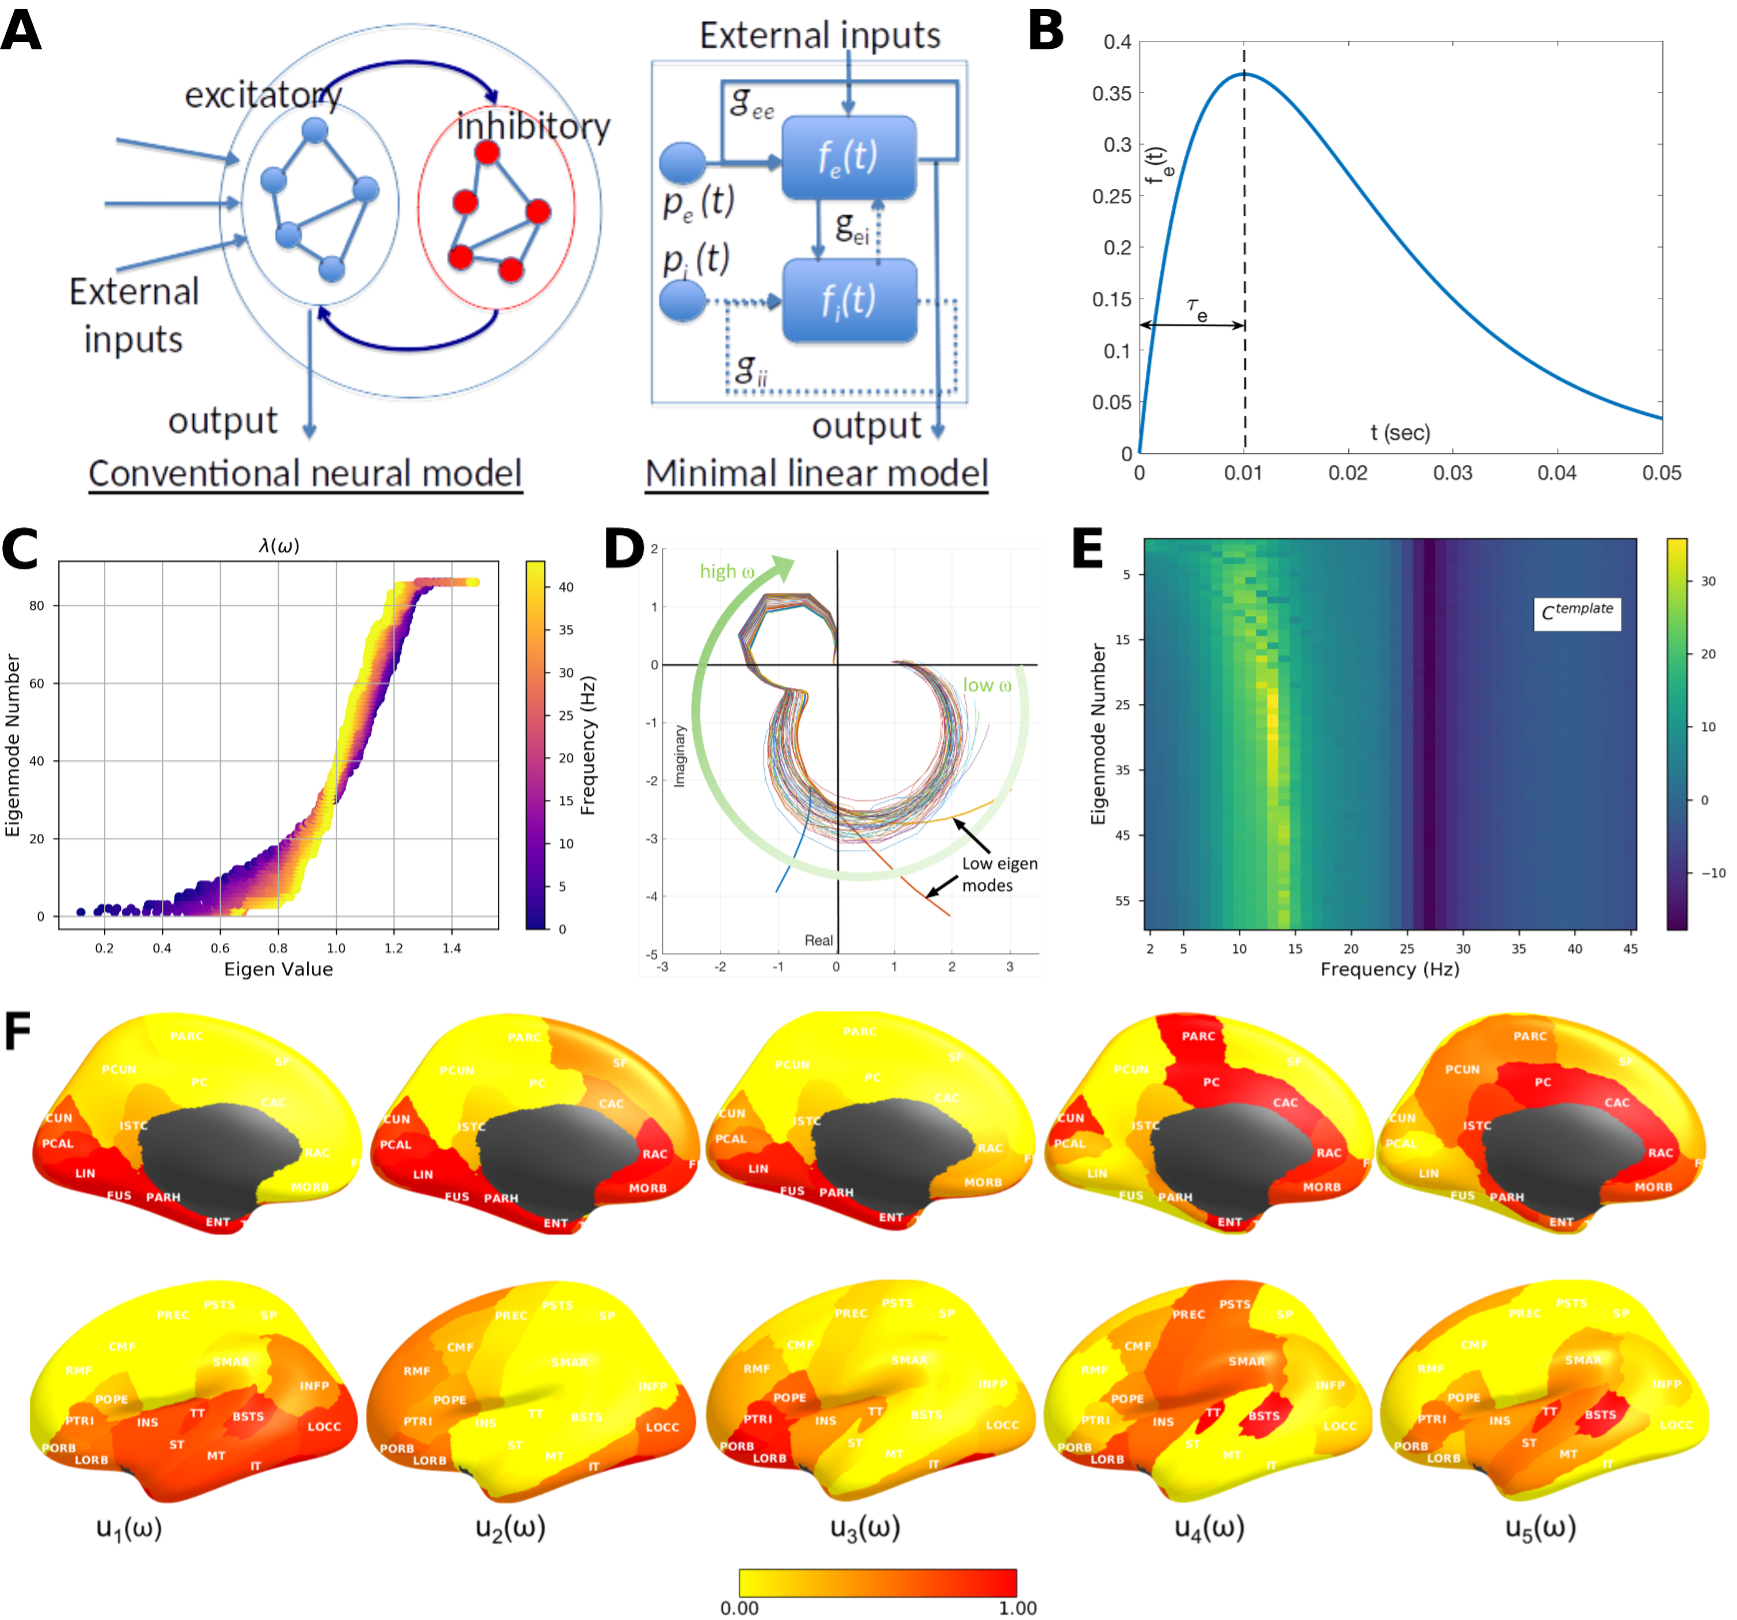
\includegraphics[scale=0.83]{../figures/chapter5/figure1.png}
    \caption{The linearized  spectral graph model.}
    \caption*{(a) Conventional neural mass models instantiate a large assembly of excitatory and inhibitory neurons, which are modeled as fully connected internally. External inputs and outputs are gated through the excitatory neurons only, and inhibitory neurons are considered strictly local. The proposed linear model condenses these local assemblies into lumped linear systems $f_{e}(t)$ and $f_{i}(t)$, Gamma-shaped functions having time constants $\tau_e$ and $\tau_i$ (see panel (b)). The recurrent architecture of the two pools within a local area is captured by the gain terms $g_{ee}$, $g_{ii}$, $g_{ei}$, parameterizing the recurrents within excitatory, inhibitory and cross-populations. (c) The absolute value of eigenvalues of the complex Laplacian $\bm{\mathcal{L}}(\omega)$ are plotted against the eigenvector index. Each dot represents one eigenvalue  $\lambda(\omega)$; its color represents the frequency $\omega$ - low (blue) to high (yellow). These eigenvalues change by frequency; small eigenvalues change more compared to large ones. (d) Frequency response of each eigenmode plotted on the complex plane with default model parameters and a template structural connectome. Each curve represents the transit in the complex plane of a single eigenmode's frequency response, starting at low frequencies in the bottom right quadrant, and moving to the upper left quadrant at high frequencies. The magnitude of the response, given by the distance from the origin, suggests that most eigenmodes have two prominent lobes, roughly corresponding to lower frequency alpha rhythms and higher frequency gamma rhythms. In contrast, the lowest eigenmodes start off far from the origin, indicative of a low-pass response. (e) Magnitude of the frequency response of each eigenmode reinforces these impressions more clearly, with clear alpha peak, as well as slower rhythms. (f) The spatial patterns of the top 5 eigenmodes of $\bm{\mathcal{L}}(\omega)$, evaluated at the alpha frequency. The first 5 eigenmodes $\bm{u}_1 ... \bm{u}_5$ produce resting-state functional networks patterns; These patterns are not exclusive and greatly depend on the frequency,  model parameters, and the connectome.}
    \label{fig:sgmodel}
\end{figure}

We applied this model to and validated its construct against measured
source-reconstructed MEG recordings in healthy subjects under rest and
eyes-closed. The model closely matches empirical spatial and spectral
MEG patterns. In particular, the model displays prominent alpha and beta
peaks, and, intriguingly, the eigenmodes corresponding to the alpha
oscillations have the same posterior-dominant spatial distribution that
is repeatedly seen in eyes-closed alpha power distributions. In contrast
to existing less parsimonious models in the literature that invoke
spatially-varying parameters or local rhythm generators, to our
knowledge, this is the first account of how the spectral graph structure
of the structural connectome can parsimoniously explain the spatial
power distribution of alpha and beta frequencies over the entire brain
measurable on MEG.

\section{Methods}

\subsection{Spectral graph model development}
\textbf{Notation}. In our notation, vectors and matrices are
represented by boldface, and scalars by normal font. We denote frequency
of a signal, in Hertz, by symbol $f$, and the corresponding angular
frequency as $(\omega = 2 \pi f$. The connectivity matrix is denoted by
$\mathbf{C} = \left\{ c_{jk} \right\}$, consisting of
connectivity strength $c_{ij}$ between any two pair of regions $j,k$.

\textbf{Model summary}: Details of the Spectral Graph model (SGM) is
described in detail below. There are very few model parameters, seven in
total:
$\tau_{e}, \tau_{i}, \tau_{G}, v, g_{ii}, g_{ei}, \alpha$,
which are all global and apply at every node. See Table \ref{tab:SGM_parameters} for
their meaning, initial value and range. Note that the entire model is
based on a single equation of graph dynamics, Eq \ref{eq:rate_model}, which is
repeatedly applied to each level of the hierarchy. Here we used two
levels: a mesoscopic level where connectivity is all-to-all, and a
macroscopic level, where connectivity is measured from fiber
architecture. In theory, this template could be refined into finer
levels, where neural responses become increasingly non-linear, and
connectivity becomes sparser and structured.



\begin{table}
  \caption{SGM parameters values and limits}
  \label{tab:SGM_parameters}
  \centering
 \begin{tabular}{m{14em}|m{2cm}|m{2cm}|m{7em}}
 \hline
 Name & Symbol & Default Value & Optimizaiton Bounds \\
 \hline
 Excitatory Time constant & $ \tau_{e}$ & 12 ms & [5ms, 20ms] \\
 Inhibitory Time constant & $\tau_{i}$ & 3 ms & [5ms, 20ms] \\
 Graph Time constant & $\tau_{G}$ & 6 ms & [5ms, 20ms] \\
 \multicolumn{4}{l}{} \\
 Excitatory gain & $g_{ee}$ & 1 & n/a \\
 Inhibitory gain & $g_{ii}$ & 1 & [0.5, 5] \\
 Excitatory gain & $g_{ei}$ & 4 & [0.5, 5] \\
 \multicolumn{4}{l}{} \\
 Transmission velocity & $v$ & 5 m/s & [5 m/s, 20 m/s] \\
 Long-range connectivity coupling constant & $\alpha$ & 1 & [0.1, 1] \\
 \end{tabular}
\end{table}


\textbf{Canonical rate model over a graph}. We use a canonical rate
model to describe neural activity across two hierarchical levels --
local cortical mesoscopic levels and long-range macroscopic levels. At
each level of the hierarchy of brain circuits, we hypothesize a simple
linear rate model of recurrent reverberatory activity given by

\begin{equation}
\label{eq:rate_model}
\frac{dx_{e/i}(t)}{dt} = - \frac{1}{\tau_{e/i}} f_{e/i}(t) * x_{e/i}(t) + \frac{1}{\tau_{e/i}} f_{e/i}(t) * \sum_{j,k} c_{jk} x_{e/i} (t - \tau_{jk}^{v} ) + p_{e/i}(t)
\end{equation}


where $x_{e/i}(t)$ is the mean signal of the excitatory/inhibitory
populations and $p_{e/i}(t)$ is internal noise source reflecting local
cortical column computations or input. The transit of signals, from
pre-synaptic membranes, through dendritic arbors and axonal projections,
is sought to be captured into ensemble average neural impulse response
functions $f_{e}(t) = \frac{t}{\tau_{e}}\exp(-\frac{t}{\tau_{e}})$
and $f_{i}(t) = \frac{t}{\tau_{i}}\exp(-\frac{t}{\tau_{i}})$
respectively. We disregard the non-linearity of the neural response,
hence the output at the terminal to a presynaptic input $u(t)$ is the
simple convolution $x_{e}(t) = f_{e}(t)*u(t)$. The neural responses
$f_{e/i}(t)$ are Gamma-shaped responses (Figure \ref{fig:sgmodel}B)
parameterized by time constants $\tau_{e/i}$ that here represent the
end result of both synaptic membrane capacitance and the distribution of
dendritic/axonal delays introduced by the arborization. NMMs typically
use a single classical exponential decay term for membrane capacitance
only, since NMMs model highly local cell assemblies where multisynaptic
connections are infrequent and axonal and dendritic transport delays are
usually incorporated explicitly via connectivity weights and delays.
Since our lumped model was designed for relatively large cortical
regions, we employ the Gamma-shaped $f_{e/i}$ to capture not just
classical membrane capacitance but also the expected diversity of
dendritic transport delays. The dynamics of the entire assembly modeled
via a self-decaying term
$\tau_{e/i} \frac{d\mathbf{x}}{dt} \propto - f_{e/i}(t) * \mathbf{x}(t)$,
typically used in most rate or NMM models, but the difference here is
that we chose to apply convolution with neural response $f_{e/i}(t)$
within the decay process. We believe this is necessary to ensure that
the dynamics of the population cannot participate in the internal
recurrent dynamics of the region until the signal has passed through one
instance of the neuronal response. Since this neural response is meant
to capture a distribution of local circuit delays, its time constants
$\tau_{e/i}$ are purposefully far longer (up to 20ms) than expected
from membrane capacitance alone. Studies of cortical lag times using
paired electrode recordings between primary and higher cortices
demonstrate this. A short visual stimulus causes a neural response in
the ferret V1 within 20ms post-stimulus, in the primary barrel field
within 16-36ms, and the entire visual cortex becomes engaged 48-70ms
after stimulus \cite{roland_tracing_2014}. Brief deflection of a single barrel
whisker in the mouse evokes a somatotopically mapped cortical
depolarization that remains localized to its C2 barrel column only for a
few milliseconds, thence rapidly spreading to a large part of
sensorimotor cortex within tens of milliseconds, a mechanism considered
essential for the integration of sensory information
\cite{ferezou_spatiotemporal_2007, polack_long-range_2012}. Interestingly, the evoked response curve in S1
from the \textsuperscript{50} study had a prominent Gamma shape. Of
note, the duration of S1 response (\textasciitilde50ms) was considerably
longer than the time to first sensory response in C2 (7.2ms)
\cite{ferezou_spatiotemporal_2007}. Interestingly, feedback projections from higher to
lower areas take \textasciitilde50ms, hence have a much slower apparent
propagation velocity (0.15-0.25m/s) than what would be predicted by
axonal conduction alone (1-3m/s) \cite{roland_tracing_2014}.

Individual neural elements are connected to each other via connection
strengths $c_{jk}$. Let the cortico-cortical fiber conduction
speed be $v$, which here is assumed to be a global constant
independent of the pathway under question. For a given pathway
connecting regions \emph{j} and \emph{k} of length $d_{jk}$,
the conduction delay of a signal propagating from region \emph{j} to region
\emph{k} will be given by
$\tau^{v}_{jk} = \frac{d_{jk}}{v}$. Hence signals from
neighboring elements also participate in the same recurrent dynamics,
giving the second term of Eq \ref{eq:rate_model}. Equation \ref{eq:rate_model} will serve
as our canonical rate model, and will be reproduced at all levels of the
hierarchy, and only the connectivity strengths will vary depending on
the level of hierarchy we are modeling, as explained below.

\textbf{Local neural assemblies}. The local connectivities
$c_{jk}^{local}$ are assumed to be all-to-all, giving a
complete graph. Further, the axonal delays $\tau_{jk}^{v}$
associated with purely local connections were already incorporated in
the lumped impulse responses $f_{e/i}(t)$. Hence, we assert:

\begin{equation}
 c_{jk}^{local} = c_{e/i},\ \ \tau_{jk}^{v} = 0,\ \forall\ j,k\
\end{equation}

From spectral graph theory, a complete graph has all equal eigenvalues
which allows the local network to be lumped into gain constants, and the
summation removed. Indeed, rewriting $x_{e/i}(t)$ as the mean signal
of all the excitatory/inhibitory cells and setting the gains $g_{ee} = 1 - c_{e} N_{e}$ and $g_{ii} = 1 - c_{i} N_{i}$ we get

\begin{equation}
\label{eq:mean_sig}
 \frac{dx_{e/i}(t)}{dt} = -\frac{g_{ee/ii}}{\tau_{e/i}} f_{e/i}(t) * x_{e/i}(t) + p_{e/i}(t)
\end{equation}

Given the Fourier Transform pairs $\frac{d}{dt} \leftrightarrow j \omega $,
$f_{e/i}(t) \leftrightarrow F_{e/i}(\omega) = \frac{1/\tau_{e/i}^{2}}{(j \omega + 1/\tau_{e/i})^{2}}$,
we take the Fourier transform of Eq \ref{eq:rate_model} and obtain the local assembly's
frequency spectrum:

\begin{equation}
\label{eq:local_fourier}
X_{e/i}(\omega) = (j \omega + \frac{g_{ee/ii}}{\tau_{e/i}} F_{e/i}(\omega))^{-1} P_{e/i} (\omega) 
\end{equation}

Writing this in terms of transfer functions
$X_{e}(\omega) = H_{e}(\omega)P_{e}(\omega), X_{i}(\omega) = H_{i}(\omega)P_{i}(\omega)$
we get the lumped local system illustrated in Figure \ref{fig:sgmodel}.
Finally, we must also account for signals that alternate between the two
populations, which is given by the transfer function

\begin{equation}
\label{eq:transfun}
H_{ei}(\omega) = H_{e}(\omega)H_{i}(\omega) / (1 + g_{ei} H_{e}(\omega) H_{i}(\omega))
\end{equation}

We fix $g_{ee} = 1$ without loss of generality, and let the
other terms $g_{ii}, g_{ei}$ be model parameters to
be fitted. Finally, the total cortical transfer function is the sum

\begin{equation}
\label{eq:cort_transfun}
H_{local}(\omega) = H_{e}(\omega) + H_{i}(\omega) + H_{ei}(\omega)
\end{equation}

and $X_{local}(\omega) = H_{local}(\omega)P(\omega)$
represents all neural activity in this region, whether from excitatory
or inhibitory cells. The canonical local activity is therefore defined
by the Fourier transform pair: $x_{local}(t) \leftrightarrow X_{local}(\omega)$.

\subsection{Macroscopic scale: signal evolution on the entire graph}
For the macroscopic level, we use the same canonical network dynamics as
Eq \ref{eq:rate_model}, but now the inter-regional connectivity $c_{jk}$ is
non-zero and given by the structural connectome. Similarly, axonal
conductance delays are determined by fiber length and conductance speed
$\tau_{jk}^{v} = d_{jk} / v$. Further, the external
driving signals at each node is the local neural activity
$x_{local}(t)$ defined above rather than a noise process
$p(t)$. In the interest of parsimony we set each node of the
macroscopic graph to have the same internal power spectrum
$X_{local}(\omega)$ - i.e. all regions are experiencing the
same transfer function, driven by identically distributed (but of course
not identical) noise. At this scale, activity measured at graph nodes is
no longer excitatory or inhibitory, but mixed, and the corticocortical
connections are all between long, pyramidal excitatory-only cells. Thus,
for the k-th node

\begin{equation}
\label{eq:node_eq}
\frac{dx_{k}(t)}{dt} = - \frac{1}{\tau_{G}}f_{e}(t) * x_{k}(t) + \frac{\alpha}{\tau_{G}} f_{e}(t) * \sum_{j} c_{jk} x_{j}(t - \tau_{jk}^{v}) + x_{local, k}(t)
\end{equation}

Here we have introduced a global coupling constant $\alpha$, similar
to most connectivity-coupled neural mass models, that seeks to control
the relative weight given to long-range afferents compared to local
signals. We have also introduced a new time constant, $\tau_{G}$,
which is an excitatory time constant and it may be the same as the
previously used constant $\tau_{e}$. However, we allow the possibility
that the long-range projection neurons might display a different
capacitance and morphology compared to local circuits, hence we have
introduced $\tau_{G}$ (subscript $G$ is for ``graph'' or ``global'').

Stacking all equations from all nodes and using vector valued signals
$\mathbf{x}(t) = { x_{k}(t)}$, we can write

\begin{equation}
\label{eq:vec_signal}
\frac{d\mathbf{x}(t)}{dt} = - \frac{1}{\tau_{G}} f_{e}(t) * \mathbf{x}(t) + \frac{\alpha}{\tau_{G}}f_{e}(t) * C\{ \mathbf{x} ( t - \tau_{jk}^{v} )\} + \mathbf{x}_{local}(t)
\end{equation}

where the braces $\{ \cdot \}$  represent all elements of a matrix
indexed by $j,k$.

We wish to evaluate the frequency spectrum of the above. In Fourier
space, delays become phases; hence we use the transform pairs
$\frac{d\mathbf{x}}{dt} \leftrightarrow j \omega \mathbf{X}(\omega)$ and
$\mathbf{x}(t - \tau) \leftrightarrow e^{- j\tau\omega}\mathbf{X}(\omega)$.
Therefore, define a "complex connectivity matrix" at any given angular
frequency $\omega$ as
$\mathbf{C}^{\mathbf{*}}(\omega) ={ c_{jk} \exp ( - j \omega \tau^{v}_{jk} ) }$.
We then define a normalized complex connectivity matrix at frequency
$\omega$ as

\begin{equation}
\label{eq:comp_conn}
\mathcal{C}(\omega) = \textrm{diag}(\frac{1}{\mathbf{\deg}}) \mathbf{C}^{\mathbf{*}}(\omega)
\end{equation}

where the degree vector $\mathbf{\deg}$ is defined as
$\deg_{k}= \sum_{j} c_{jk}$. Taking the Fourier transform
of Equation \ref{eq:vec_signal}, we get

\begin{equation}
\label{eq:fourier_sig}
(j \omega \mathbf{X}(\omega) + \frac{1}{\tau_{G}} F_{e}(\omega) (\mathbf{I} - \alpha \mathcal{C}(\omega)) \mathbf{X}(\omega)) = H_{local}(\omega) \mathbf{P}(\omega) 
\end{equation}

where we assumed identically distributed noise signals driving both the
excitatory and inhibitory local populations at each node, such that
$P_{e,k}(\omega) = P_{i,k}(\omega) = P_{k}(\omega)$ at the $k$-th node.
We then collected all nodes' driving inputs in the vector
$\mathbf{P}(\omega) = { P_{k}(\omega), \forall k }$.
Here, we define the complex Laplacian matrix

\begin{equation}
\label{eq:clap}
\mathcal{L}(\omega) = \mathbf{I} - \alpha \mathcal{C}(\omega)
\end{equation}

where $\mathbf{I}$ is the identity matrix of size $N \times N$. This
complex Laplacian will be evaluated via the eigen-decomposition

\begin{equation}
\label{eq:decomp}
\mathcal{L}(\omega) = \mathbf{U}(\omega)\mathbf{\Lambda}(\omega)\mathbf{U}(\omega)^{H}
\end{equation}

where
$\mathbf{\Lambda}(\omega) = \textrm{diag}([\lambda_{1}(\omega),\ldots,\lambda_{N}(\omega)])$
is a diagonal matrix consisting of the eigenvalues of the complex
Laplacian matrix of the connectivity graph $\mathcal{C}(\omega)$, at
the angular frequency $\omega$.

Hence
\begin{equation}
\label{eq:lap_sgm}
\mathbf{X}(\omega) = (j\omega\mathbf{I} + \frac{1}{\tau_{G}} F_{e}(\omega) \mathcal{L}(\omega))^{-1} H_{local}(\omega)\mathbf{P}(\omega)
\end{equation}

where we invoke the eigen-decomposition of $\mathcal{L}(\omega)$, and
that $\mathbf{U}(\omega){\mathbf{U}(\omega)}^{H} = \mathbf{I}$. It
can then be shown easily that

\begin{equation}
\label{eq:sgm}
\mathbf{X}(\omega) =\sum_{i}\frac{\mathbf{u}_{i}(\omega)\mathbf{u}_{i}^{H}(\omega)}{j\omega + \frac{1}{\tau_{G}}\lambda_{i}(\omega) F_{e}(\omega)} H_{local}(\omega) \mathbf{P}(\omega)
\end{equation}

This is the steady state frequency response of the whole brain dynamics.
In steady state, we assume that each cortical region is driven by
internal noise that spans all frequencies, i.e. white noise. Hence, we
assume that the driving function $\mathbf{p}(t)$ is an uncorrelared
Gaussian noise process, such that
$\mathbf{P}(\omega) = \mathbb{I}$ where $\mathbb{l}$ is a vector of
ones. This asserts identical cortical responses at each brain region.

\subsection{Experimental Procedures}
\textbf{Study cohort}. We acquired MEG, anatomical MRI, and diffusion
MRI for 36 healthy adult subjects (23 males, 13 females; 26 left-handed,
10 right-handed; mean age 21.75 years (range: 7-51 years). All study
procedures were approved by the institutional review board at the
University of California at San Francisco (UCSF) and are in accordance
with the ethics standards of the Helsinki Declaration of 1975 as revised
in 2008.

\textbf{MRI.} A 3 Tesla TIM Trio MR scanner (Siemens, Erlangen,
Germany) was used to perform MRI using a 32-channel phased-array
radiofrequency head coil. High-resolution MRI of each subject's brain
was collected using an axial 3D magnetization prepared rapid-acquisition
gradient-echo (MPRAGE) T1-weighted sequence (echo time {[}TE{]} = 1.64
ms, repetition time {[}TR{]} = 2530 ms, TI = 1200 ms, flip angle of 7
degrees) with a 256-mm field of view (FOV), and 160 1.0-mm contiguous
partitions at a 256×256 matrix. Whole-brain diffusion weighted images
were collected at b = 1000$s/mm^{2}$ with 30 directions using 2-mm
voxel resolution in-plane and through-plane.

\textbf{Magneto-encephalography (MEG) data}. MEG recordings were
acquired at UCSF using a 275-channel CTF Omega 2000 whole-head MEG
system from VSM MedTech (Coquitlam, BC, Canada). All subjects were
instructed to keep their eyes closed for five minutes while their MEGs
were recorded at a sampling frequency of 1200 Hz.

\subsection{Data Processing}

\textbf{Region Parcellations}. The T1-weighted images were parcellated
into 68 cortical regions and 18 subcortical regions using the using the
Desikan-Killiany atlas available in the FreeSurfer software
\cite{Fischl2002}. To do this, the subject specific T1-weighted
images were back-projected to the atlas using affine registration, as
described in our previous studies \cite{abdelnour_network_2014,owen_structural_2013}.

\textbf{Structural Connectivity Networks.} We constructed different
structural connectivity networks with the same Desikan-Killiany
parcellations to access the capabilities of our proposed model. Firstly,
we obtained openly available diffusion MRI data from the MGH-USC Human
Connectome Project to create an average template connectome. As in our
previous studies \cite{abdelnour_network_2014,owen_structural_2013}, subject specific structural
connectivity was computed on diffusion MRI data: \emph{Bedpostx} was
used to determine the orientation of brain fibers in conjunction with
\emph{FLIRT}, as implemented in the \emph{FSL} software
\cite{Jenkinson2012}. In order to determine the elements of the
adjacency matrix, we performed tractography using \emph{probtrackx2}. We
initiated 4000 streamlines from each seed voxel corresponding to a
cortical or subcortical gray matter structure and tracked how many of
these streamlines reached a target gray matter structure. The weighted
connection between the two structures $c_{i,j}$, was defined as the
number of streamlines initiated by voxels in region $i$that
reach any voxel within region $j$, normalized by the sum of the source
and target region volumes
($c_{i,j} = \frac{\textrm{streamlines}}{v_{i} + v_{j}}$). This
normalization prevents large brain regions from having high connectivity
simply due to having initiated or received many streamlines. Afterwards,
connection strengths are averaged between both directions ($c_{i,j}$
and $c_{j,i}$) to form undirected edges. It is common in neuroimaging
literature to threshold connectivity to remove weakly connected edges,
as this can greatly influence the implied topology of the graph. In our
work, we chose not to apply further thresholding, as unlike conventional
graph theoretic metrics, linear models of spread and consequently
network eigenmodes are relatively insensitive to implied topology
induced by presence (or lack) of weak nonzero connections. However, to
determine the geographic location of an edge, the top 95\% of non-zero
voxels by streamline count were computed for both edge directions. The
consensus edge was defined as the union between both post-threshold
sets.

\textbf{MEG processing and source reconstruction.} MEG recordings were
down-sampled from 1200 Hz to 600 Hz, then digitally filtered to remove
DC offset and any other noisy artifact outside of the 1 to 160 Hz
bandpass range. Since MEG data are in sensor space, meaning they
represent the signal observable from sensors placed outside the head,
this data needs to be ``inverted'' in order to infer the neuronal
activity that has generated the observed signal by solving the so-called
inverse problem. Several effective methods exist for performing
\emph{source localization} \cite{wipf_robust_2010,zumer_probabilistic_2008,jerbi_localization_2004}. Here we eschew the
common technique of solving for a small number of discrete dipole
sources which is not fully appropriate in the context of inferring
resting state activity, since the latter is neither spatially sparse not
localized. Instead, we used adaptive spatial filtering algorithms from
the NUTMEG software tool written in house \cite{dalal_nutmeg_2004} in MATLAB
(The MathWorks, Inc., Natick, Massachusetts, United States). To prepare
for source localization, all MEG sensor locations were co-registered to
each subject's anatomical MRI scans. The lead field (forward model) for
each subject was calculated in NUTMEG using a multiple local-spheres
head model (three-orientation lead field) and an 8 mm voxel grid which
generated more than 5000 dipole sources, all sources were normalized to
have a norm of 1. Finally, the MEG recordings were projected into source
space using a beamformer spatial filter. Source estimates tend to have a
bias towards superficial currents and the estimates are more error-prone
when we approach subcortical regions, therefore, only the sources
belonging to the 68 cortical regions were selected to be averaged around
the centroid. Specifically, all dipole sources were labeled based on the
Desikan-Killiany parcellations, then sources within a 20 mm radial
distance to the centroid of each brain region were extracted, the
average time course of each region's extracted sources served as
empirical resting-state data for our proposed model.

\textbf{Alternative benchmark model for comparison.} In order to put the
proposed model in context, we also implemented for comparison a
Wilson-Cowan neural mass model \cite{destexhe_wilson-cowan_2009,wilson_mathematical_1973,muldoon_stimulation-based_2016} (add criticism citation here) with
similar dimensionality. Although NMMs like this can and have been
implemented with regionally varying local parameters, here we enforced
uniform, regionally non-varying local parameters, meaning all
parcellated brain regions shared the same local and global parameters.
This is a fair comparison since the proposed model is also regionally
non-varying. The purpose of this exercise is to ascertain whether a
non-regional NMM can also predict spatial power variations purely as a
consequence of network transmission, like the proposed model, using the
same model optimization procedure (see below). This NMM incorporates a
transmission velocity parameter that introduces a delay based on fiber
tract lengths extracted from diffusion MRI, but, unlike our model, does
not seek to explicitly evaluate a frequency response based on these
delays.

\subsection{Model Optimization}
We computed \emph{maximum a posteriori} estimates for parameters under a
flat non-informative prior. A simulated annealing optimization algorithm
was used for estimation and provided a set of optimized parameters
$\{\tau_{e}, \tau_{i}, \tau_{c}, g_{ei}, g_{ii}, \alpha, \upsilon\}$.
We defined a data likelihood or goodness of fit (GOF) as the Pearson
correlation between empirical source localized MEG power spectra and
simulated model power spectra, averaged over all 68 regions of a
subject's brain. The proposed model has only seven global parameters as
compared to neural mass models with hundreds of parameters, and is
available in closed-form. To improve the odds that we capture the global
minimum, we chose to implement a probabilistic approach of simulated
annealing \cite{Kirkpatrick1983}. The algorithm samples a set of
parameters within a set of boundaries by generating an initial trial
solution and choosing the next solution from the current point by a
probability distribution with a scale depending on the current
"temperature" parameter. While the algorithm always accepts new trial
points that map to cost-function values lower than the previous
cost-function evaluations, it will also accept solutions that have
cost-function evaluations greater than the previous one to move out of
local minima. The acceptance probability function is
$1/(1 + \frac{\mathrm{\Delta}}{e^{\max(T)}})$, where T is the current
temperature and $\Delta$ is the difference of the new minus old cost-function
evaluations. The initial parameter values and boundary constraints for
each parameter are given in Table \ref{tab:SGM_parameters}. All simulated
annealing runs were allowed to iterate over the parameter space for a
maximum of $N_{p} \times 3000$ iterations, where $N_{p}$ is the
number of parameters in the model. As a comparison, we performed the
same optimization procedure to a regionally non-varying Wilson-Cowan
neural mass model \cite{wilson_mathematical_1973,muldoon_stimulation-based_2016}.

\section{Results}
\subsection{Graph Laplacian eigenmodes mediate a diversity of frequency
responses}

First, we demonstrate the spectra produced by graph eigenmodes as per
our theory using default choices of model parameters. Figure \ref{fig:sgmodel}C
shows the eigen-spectrum of the complex Laplacian, with eigenvalue
magnitude ranging from 0 to 1. The absolute value of eigenvalues of the
complex Laplacian $\mathcal{L}(\omega)$ are plotted against the
eigenvector index. Each dot represents one eigenvalue
$\lambda(\omega)$; its color represents the frequency $\omega$ - low
(blue) to high (yellow). Clearly, these eigenvalues change somewhat by
frequency. Small eigenvalues undergo a larger shift due to frequency,
while the large ones stay more stable and tightly clustered around the
nominal eigenvalue (i.e. at $\omega = 0$). Each eigenmode produces a
frequency response based on its frequency-dependent eigenvalue
(Figure \ref{fig:sgmodel}D, E). Figure \ref{fig:sgmodel}D shows the transit in the
complex plane of a single eigenmode's frequency response, starting at
low frequencies in the bottom right quadrant, and moving to the upper
left quadrant at high frequencies. The magnitude, given by distance from
origin, suggests that most eigenmodes have two prominent lobes, one
roughly corresponding to lower frequency alpha rhythm and another
corresponding to higher frequency beta or gamma rhythms, respectively.
In contrast, the lowest few eigenmodes start off far from the origin,
indicative of a low-pass response. The magnitude of these complex-valued
curves shown in Figure \ref{fig:sgmodel}E reinforces these impressions, with clear alpha
peak, as well as slower rhythms of the lowest eigenmodes. The spectral
profile of the eigenmodes, especially the peak frequencies, are
sensitive to the choice of model parameters as demonstrated below.

\begin{figure}[htbp]
    \centering
    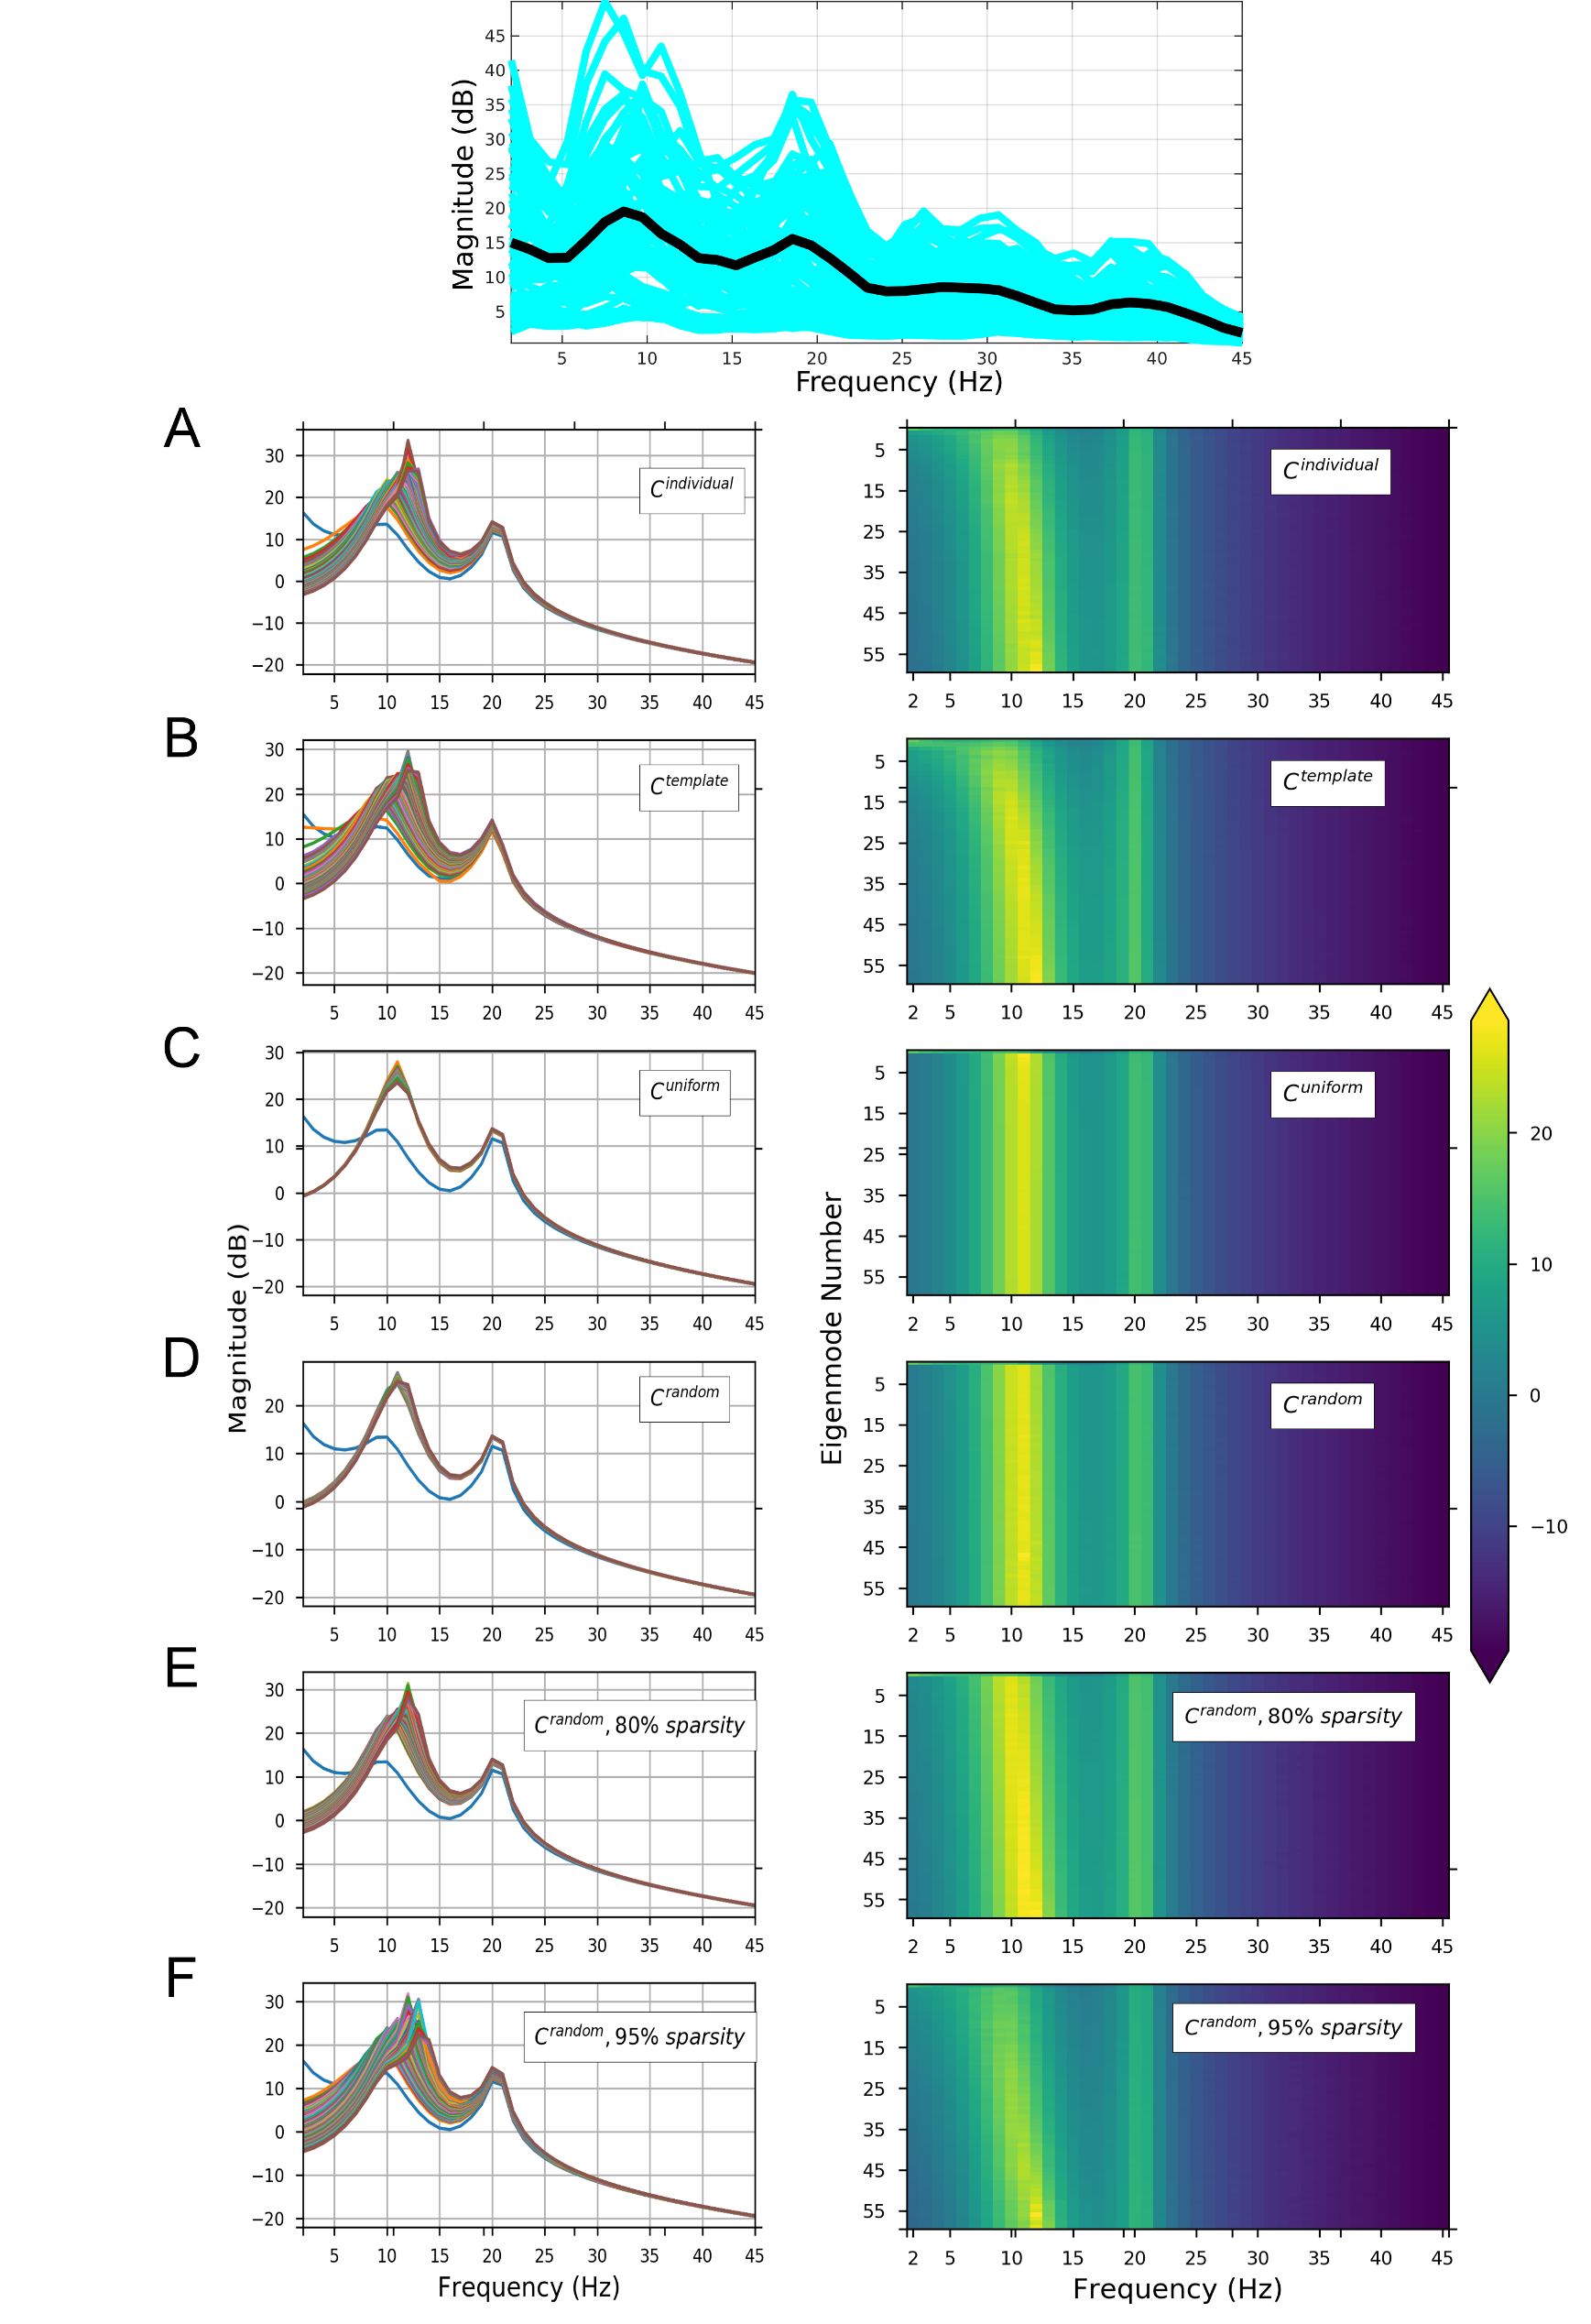
\includegraphics[scale=0.81]{../figures/chapter5/fig2_conn_spectra.png}
    \caption{Spectral graph model spectra for one subject.}
    \caption*{Top-Source localized MEG power spectrum for 68 parcellated brain regions. Estimated spectra for each brain region are shown in blue, and average spectrum across all regions is shown in black. The subsequent rows show each eigenmode's spectral magnitude response with model parameters optimized to match the MEG spectrum $(\tau_e = 0.0073, \tau_i = 0.0085, \tau_G = 0.0061, g_{ei} = 2.9469, g_{ii} = 4.4865, v = 18.3071, and \alpha = 0.4639)$. Left column shows each eigenmode's frequency responses, while the right column shows the same information as heatmaps. (a) Model using  subject's individual structural connectome. (b) Model using average template connectome obtained from 80 HCP subjects. (c) Model using uniform connectivity matrix of ones. (d) Model using randomized connectivity matrix with 75\% sparsity. (f) Model using randomized connectivity matrix with 95\% sparsity.}
    \label{fig:conn_spectra}
\end{figure}

The spatial patterns of the first 5 eigenmodes of
$\mathcal{L}(\omega)$, evaluated at the alpha peak of 10 Hz, are shown
in Figure \ref{fig:sgmodel}F. Eigenmodes
$\mathbf{u}_{\mathbf{1 - 4}}$ produce posterior and temporal spatial
patterns, including many elements of the \textbf{default mode network;}
\(\mathbf{u}_{\mathbf{4}}\) resembles the \textbf{sensorimotor network};
and \(\mathbf{u}_{5}\) the \textbf{structural core} of the human
connectome. However, these patterns are not exclusive and greatly depend
on the frequency at which they are evaluated, as well as the model
parameters. Higher eigenmodes are especially sensitive to axonal
velocity and frequency (not shown here).

Since the spectral graph model (SGM) relies on connectome topology, we
demonstrate in Figure \ref{fig:conn_spectra} that different connectivity matrices
produce different frequency responses: A) the individual's structural
connectivity matrix, B) HCP average template connectivity matrix, C)
uniform connectivity matrix of ones, D) a randomly generated matrix, E)
and F) are randomly generated matrices with 75\% and 95\% sparsity
respectively. For Figure \ref{fig:conn_spectra}A, optimized parameters for the individual
subject's connectome were used. For Figures \ref{fig:conn_spectra}B-F, parameters optimized
for the HCP template were used. We can observe the spectral profile of
the eigenmodes, especially the peak frequencies, are sensitive to the
choice of the connectome and the model parameters. All modeled power
spectra show a broad alpha peak at around 10 Hz and a narrower beta peak
at around 20 Hz. This is expected, since these general spectral
properties are governed by the local linearized rate model. It is
important to note that different eigenmodes accommodate a diversity of
frequency responses; for instance, the lowest eigenmodes show a
low-frequency response with no alpha peak whatsoever. In all cases the connectome modulates the spectral response in delta-theta range, leaving the higher gamma frequencies unchanged. Particularly, the low eigenmodes ($\mathbf{u}_1 \ldots \mathbf{u}_{20}$) appear to modulate the lower frequency range, up to beta, and may be considered responsible for the diversity of spectra observed in the model. In the frequency
responses from biologically realistic individual and HCP template
connectomes, there is a diversity of spectral responses amongst
eigenmodes that is lacking in the response produced by the unrealistic
uniform and randomized connectivity matrices. As we will see below, graph topology is
critical to the power spectrum it induces, hence we explored whether and
how sparsity of random graphs mediates spectral power (Figure \ref{fig:conn_spectra}D-F). At incrementally increasing sparsity levels, the diversity of
spectral responses of different eigenmodes increases and approaches that
of realistic connectomes. Therefore, graph eigenmodes induce unique and
diverse frequency responses that depend on the topology of the graph.

\subsection{Spectral distribution of MEG power depends on model parameters but not
connectivity}

\begin{figure}[htbp]
    \centering
    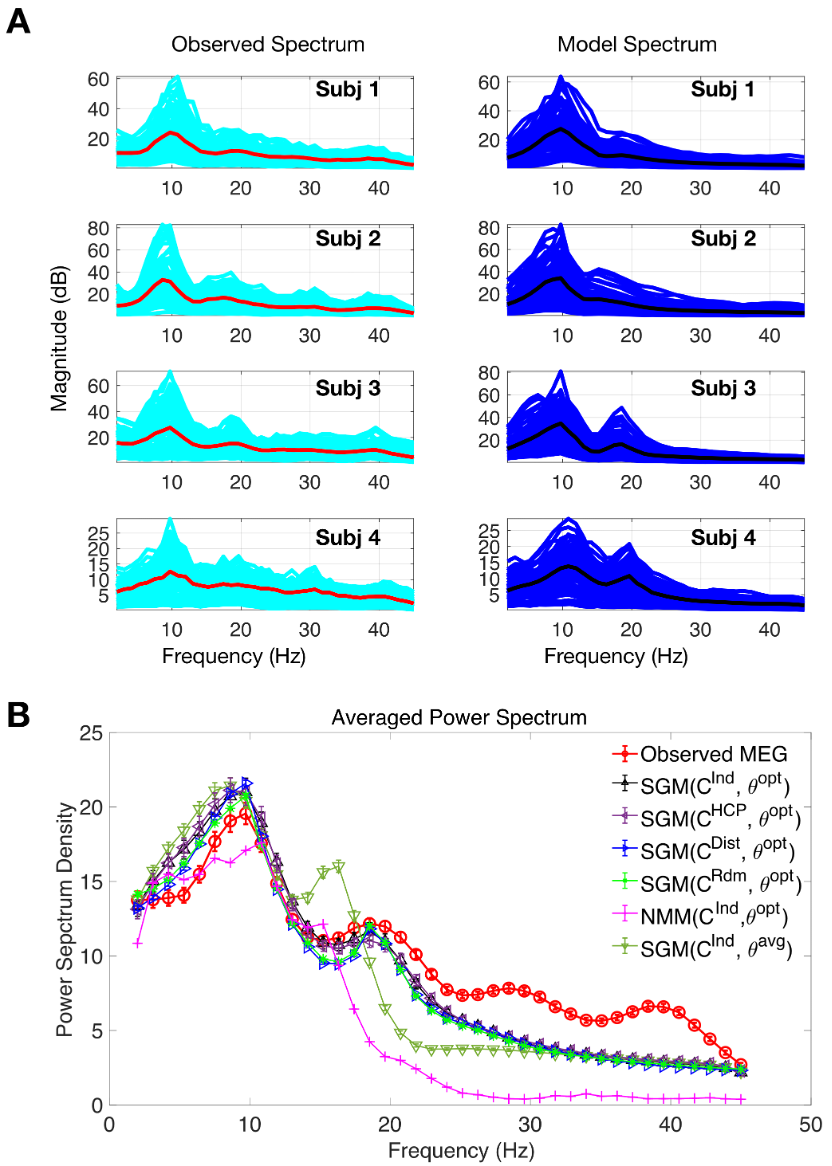
\includegraphics[scale=0.85]{../figures/chapter5/fig3_spectra_fit.png}
    \caption{Spectral graph model depicts MEG spectra.}
    \caption*{(a) The observed spectra and SGM's simulated spectra for four representative subjects. Red and cyan curves illustrate source localized empirical average spectra and region-wise spectra respectively. Black and blue curves illustrate simulated average spectra and region-wise spectra respectively. (b) Average observed spectrum across subjects is shown in red. Subsequently, we show average simulated spectra with optimized parameters for individual subject connectomes (black), HCP template connectome (purple), 80\% sparse distance connectome (blue), 80\% sparse random connectome (green). As a comparison, we also show simulated spectrum with a network neural mass model (pink) and average parameter values and individual connectome (green).}
    \label{fig:spectra_fit}
\end{figure}

Network eigenmodes exhibit strong spatial patterning in their frequency
responses, even with identical model parameters (Figure \ref{fig:spectra_fit}). We
evaluated the model spectral response using the subject-specific
$C^{ind}$ matrices of 4 representative subjects
(Figure \ref{fig:spectra_fit}A). The model power spectra strikingly
resemble empirical MEG spectra, displaying both the alpha and beta peaks
on average, and similar regional variability as in real data.

Regional averages of empirical and modeled power spectra of the entire
group after full parameter optimization over individual subjects are
shown in Figure \ref{fig:spectra_fit}B. The model closely replicates the observed
power spectrum (red circles) equally well with both $C^{ind}$
(black triangles) and $C^{HCP}$ (purple triangles). Thus, in
most cases we can safely replace the subject-specific connectome with
the template connectome. In contrast, when non-optimized average
parameters were used (golden green triangles), it resulted in a worse
fit, especially at high frequencies, suggesting that individualized
parameter optimization is essential to produce realistic spectra. We
also examined the model behavior for a random connectomes with 80\%
sparsity (bright green triangles), or a distance-based connectome (blue
triangles) was chosen with identical sparsity (80\%) to the actual
connectome, and found that even with optimized parameters the average
spectra could be accounted for by these connectomes.

As another benchmark for comparison, a non-linear network neural mass model
\cite{Wilson1972,muldoon_stimulation-based_2016} (add criticism paper) using our in-house MATLAB implementation, was generally able to produce characteristic alpha
and beta frequency peaks, but this model does not resemble empirical
wideband spectra. Note that no regionally-varying NMM parameters were
used in order to achieve a proper comparison with our model, but both
models were optimized with the same algorithm.

\begin{figure}[htbp]
    \centering
    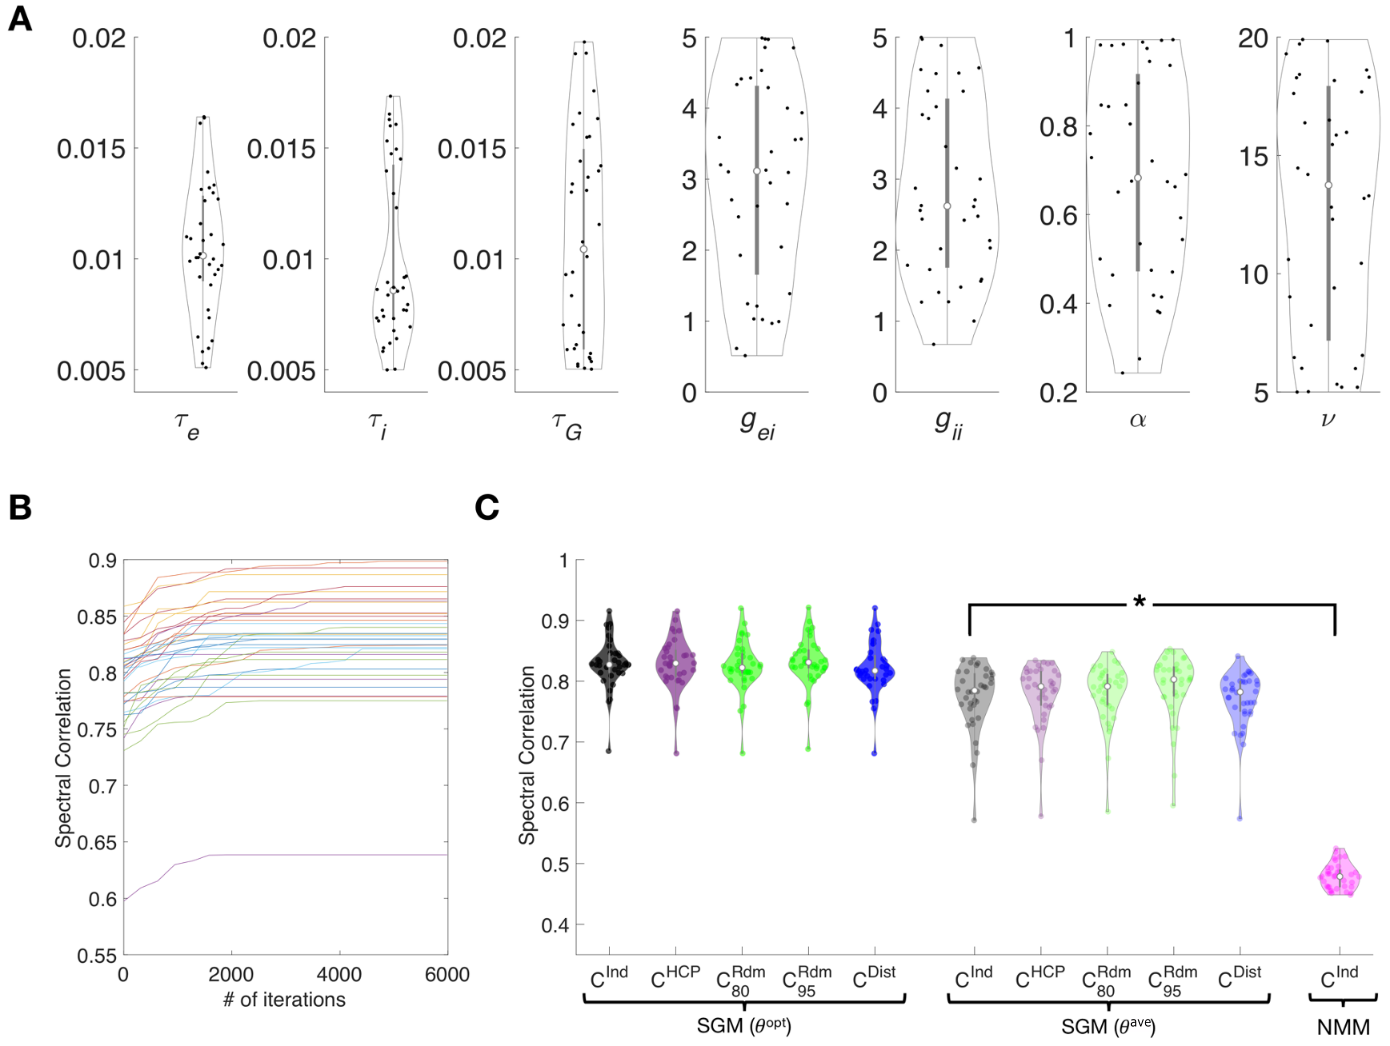
\includegraphics[width=\textwidth]{../figures/chapter5/fig4_violin.png}
    \caption{Spectral graph model parameter optimization.}
    \caption*{(a) Distribution of optimized model parameter values across all 36 subjects for parameters $\{\tau_e, \tau_i, \tau_c, g_{ei}, g_{ii}, \alpha, v\}$ are shown in violin plots. (b) Performance of optimization algorithm. Spectral Pearson's correlation between simulated and MEG spectra at each iteration. Each curve shows the spectral correlation achieved by the model optimized for a single subject. (c) Distribution of spectral correlation between optimized model and observed spectra across subjects. Correlations with optimized parameters and 5 various connectomes are shown in the left-most columns. Correlations with average parameter values and the same connectomes are shown in the middle section. SGM model outperforms an optimized network NMM regardless of connectome type as denoted by asterisk $(p < 0.001)$.}
    \label{fig:violin}
\end{figure}

Figure \ref{fig:violin}A shows violin plots of the optimized values,
indicating that there is a large range of individually optimal model
parameters across subjects. The time constants $\tau_{e}, \tau_{i}$
showed tight clustering but the rest of the parameters showed high
variability across subjects. The optimal parameters are in a
biologically plausible range, similar to values reported in numerous
neural mass models. The optimization algorithm aimed to maximize a cost
function proportional to the posterior likelihood of the model, and was
quantified by the Pearson's correlation between MEG and modeled spectra
("Spectral correlation"). The convergence plots shown in
Figure \ref{fig:violin}B, one curve for each subject, indicates substantial
improvement in cost function from default choice as optimization
proceeds. The distribution of optimized spectral correlations is shown
in Figure \ref{fig:violin}C. Other model choices were evaluated for comparison: SGM
on random connectomes with 80 and 95\% sparsity, with and without a
distance effect described in Methods, and SGM applied with average
optimal model parameters instead of individually optimized ones. In
order to test for significance, Fisher's R to z transform was applied,
followed by a paired t-test across all subjects between the optimal SGM
and other models. The spectral fits for an SGM model with individual
connectomes were significantly better than SGM models with average
parameters, no matter what connectomes were chosen $(p<0.001)$.
Interestingly, spectral fits for SGM model were comparable across all
connectomes $(p >.05)$. Furthermore, spectral fits for the SGM
model were significantly better than that for NMM models with optimized
parameters and individual connectome $(p < 1e^{-20})$. Therefore, we
conclude that with the graph spectral model, the overall regional
spectra appear to be dependent on global model parameters rather than on
the actual structural connectome.

\subsection{Spectral graph model recapitulates the spatial distribution of
MEG power}

Next, we establish that the model is able to reproduce region-specific
spectra, even though it uses identical local oscillations. We integrated
the spectral area in the range 8-12 Hz for alpha and 13-25 Hz for beta,
of each brain region separately. We define "\emph{spatial
correlation}" (as compared to spectral correlation above) as Pearson's
R between the \emph{regional distribution} of empirical MEG and
model-predicted power within a given frequency band.

\subsubsection{Small number of eigenmodes capture spatial distributions of
alpha and beta band activity}.

\begin{figure}[htbp]
    \centering
    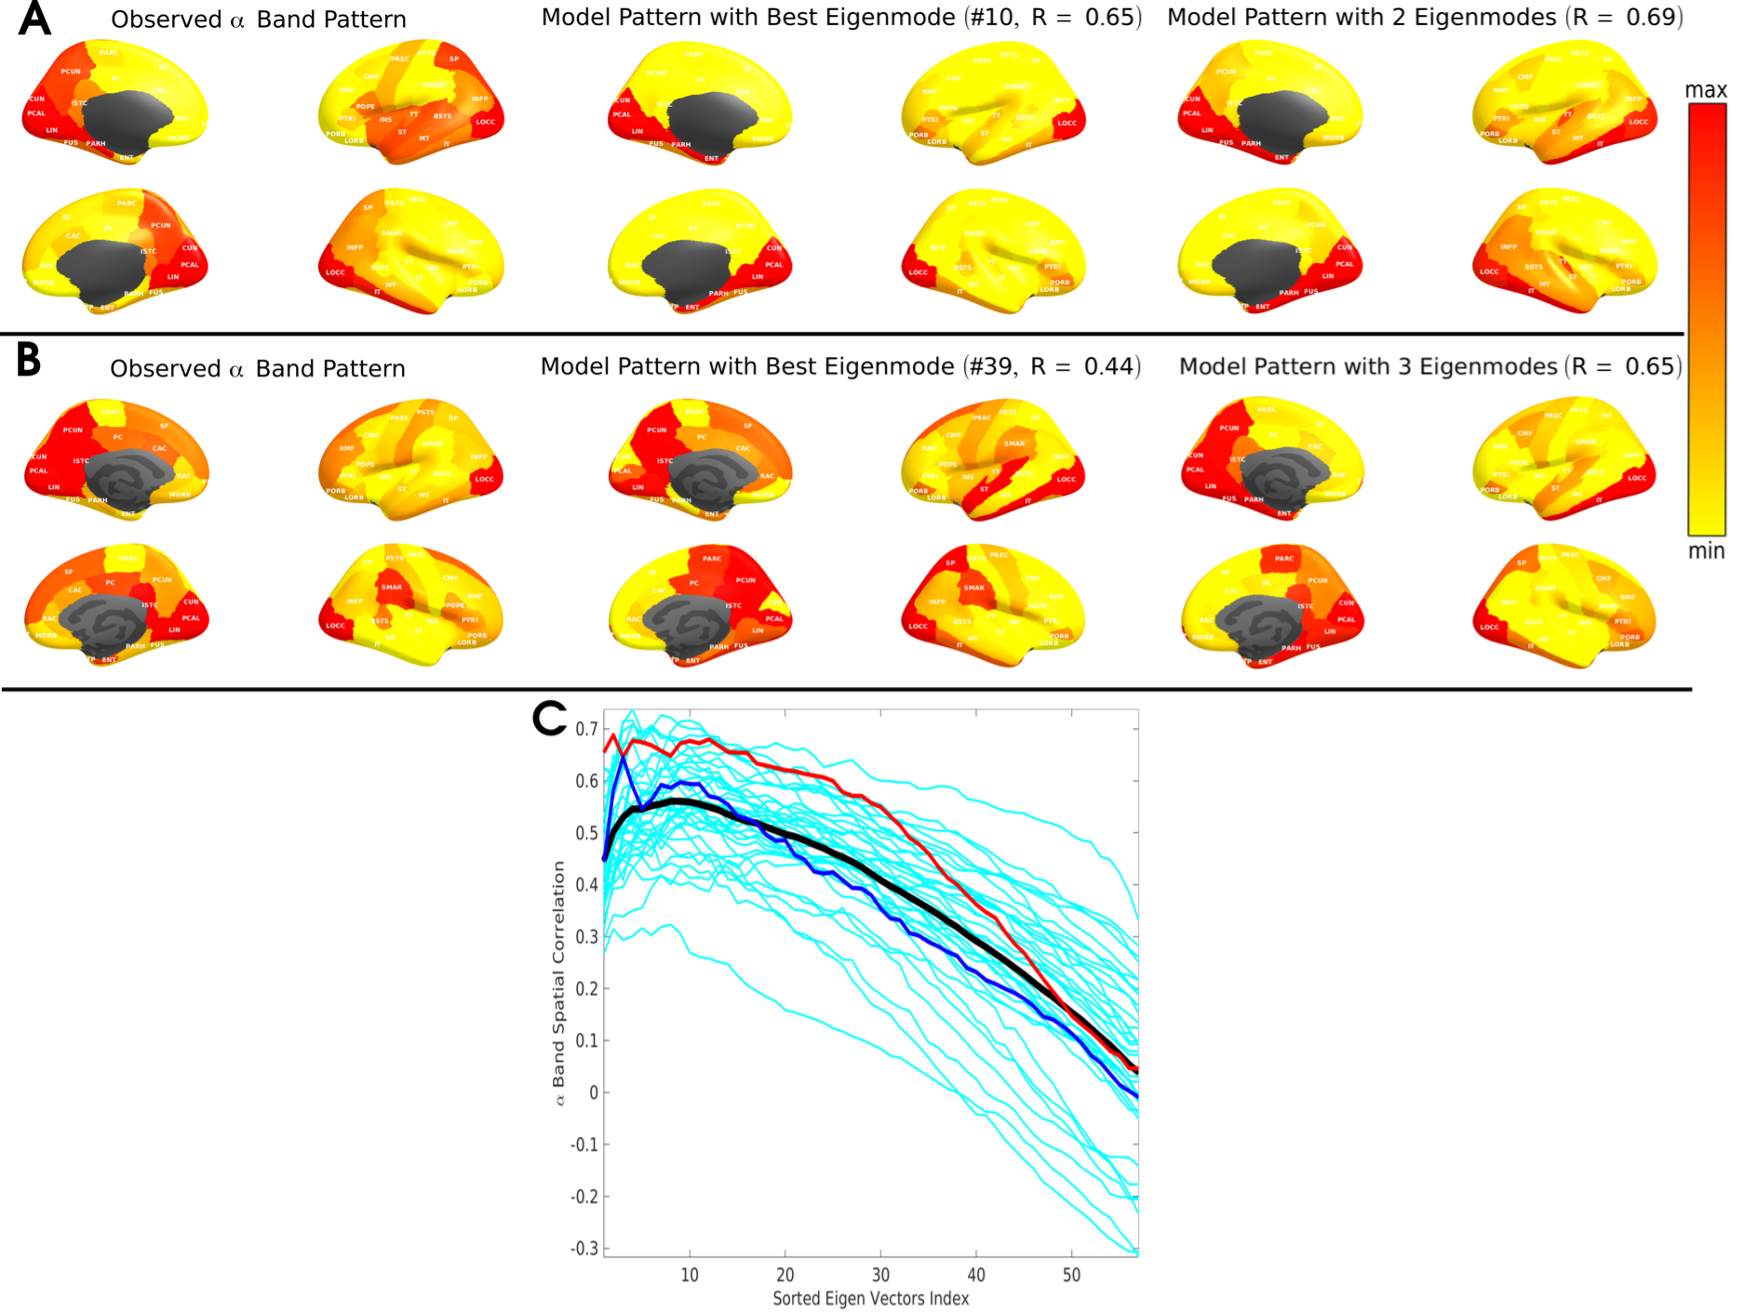
\includegraphics[width=\textwidth]{../figures/chapter5/fig5_alpha.png}
    \caption{Alpha power spatial distribution depicted by specific spectral graph model eigenmodes.}
    \caption*{(a,b) The spatially distributed patterns of alpha band power for two representative subjects are displayed in brain surface renderings. For each three brain panels shown, the medial surface rendering is shown on the left column while the lateral surface is rendered on the right, the left hemisphere is shown on top and the right hemisphere is shown in the bottom row. Left column: The observed MEG alpha band spatial distribution showing higher power in posterior regions of the brain. Middle column: Spatial distribution of the best matching eigenmode from the SGM. Right column: Spatial distribution of the best cumulative combination of eigenmodes from the SGM. (c) Alpha band spatial correlation for all subjects from SGM simulations with increasing number of cumulative eigenmodes. Individual subject alpha band spatial correlations are shown in cyan $(n=36)$. Panels A and B correspond to the subjects indicated by red and blue curves respectively. Black curve is the average performance across all subjects.}
    \label{fig:alpha}
\end{figure}

We noticed during our experimentation that only a few eigenmodes appear
to contribute substantially to observed MEG alpha and beta patterns.
Hence we hypothesized that spatial correlations could be improved by
selecting a small subset of eigenmodes. Therefore, we developed a
sorting strategy whereby we first rank the eigenmodes in descending
order of spatial correlation for a given subject and given frequency
band. Then we perform summation over only these eigenmodes according to
Eq \ref{eq:sgm}, each time incrementally adding a new eigenmode to the sum. The
spatial correlation of these "sorted-summed" eigenmodes against
empirical alpha power are plotted in Figure \ref{fig:alpha}C as a function of
increasing number of eigenmodes; one curve for each subject. The thick
black curve represents the average over all subjects. The spatial
correlation initially increases as we add more well-fitting eigenmodes,
but peaks around, and begins declining thereafter. Addition of the
remaining eigenmodes only serves to reduce the spatial correlation. This
behavior is observed in almost all subjects we studied.

Examples of predicted alpha patterns: Figure \ref{fig:alpha} shows brain
surface renderings of the spatially distributed patterns of alpha band
power for two representative subjects. Regions are color coded as a
heatmap of regional power scaled by mean power over all regions. The
observed MEG spatial distribution pattern of alpha band shows higher
power in posterior regions of the brain, as expected, with strong effect
size in temporal, occipital and medial posterior areas. This pattern is
matched by one of the eigenmodes (\#10, shown in middle panel, giving
$R=0.65$), and slightly better by a weighted combination of 2 eigenmodes
($R=0.69$). However, the model did not reproduce parietal and
parieto-occipital components seen in real data. The other subject
produced similar results, but with 6 eigenmodes. In this instance, the
parietal component seen in real data were reasonably reproduced by the
model.

\begin{figure}[htbp]
    \centering
    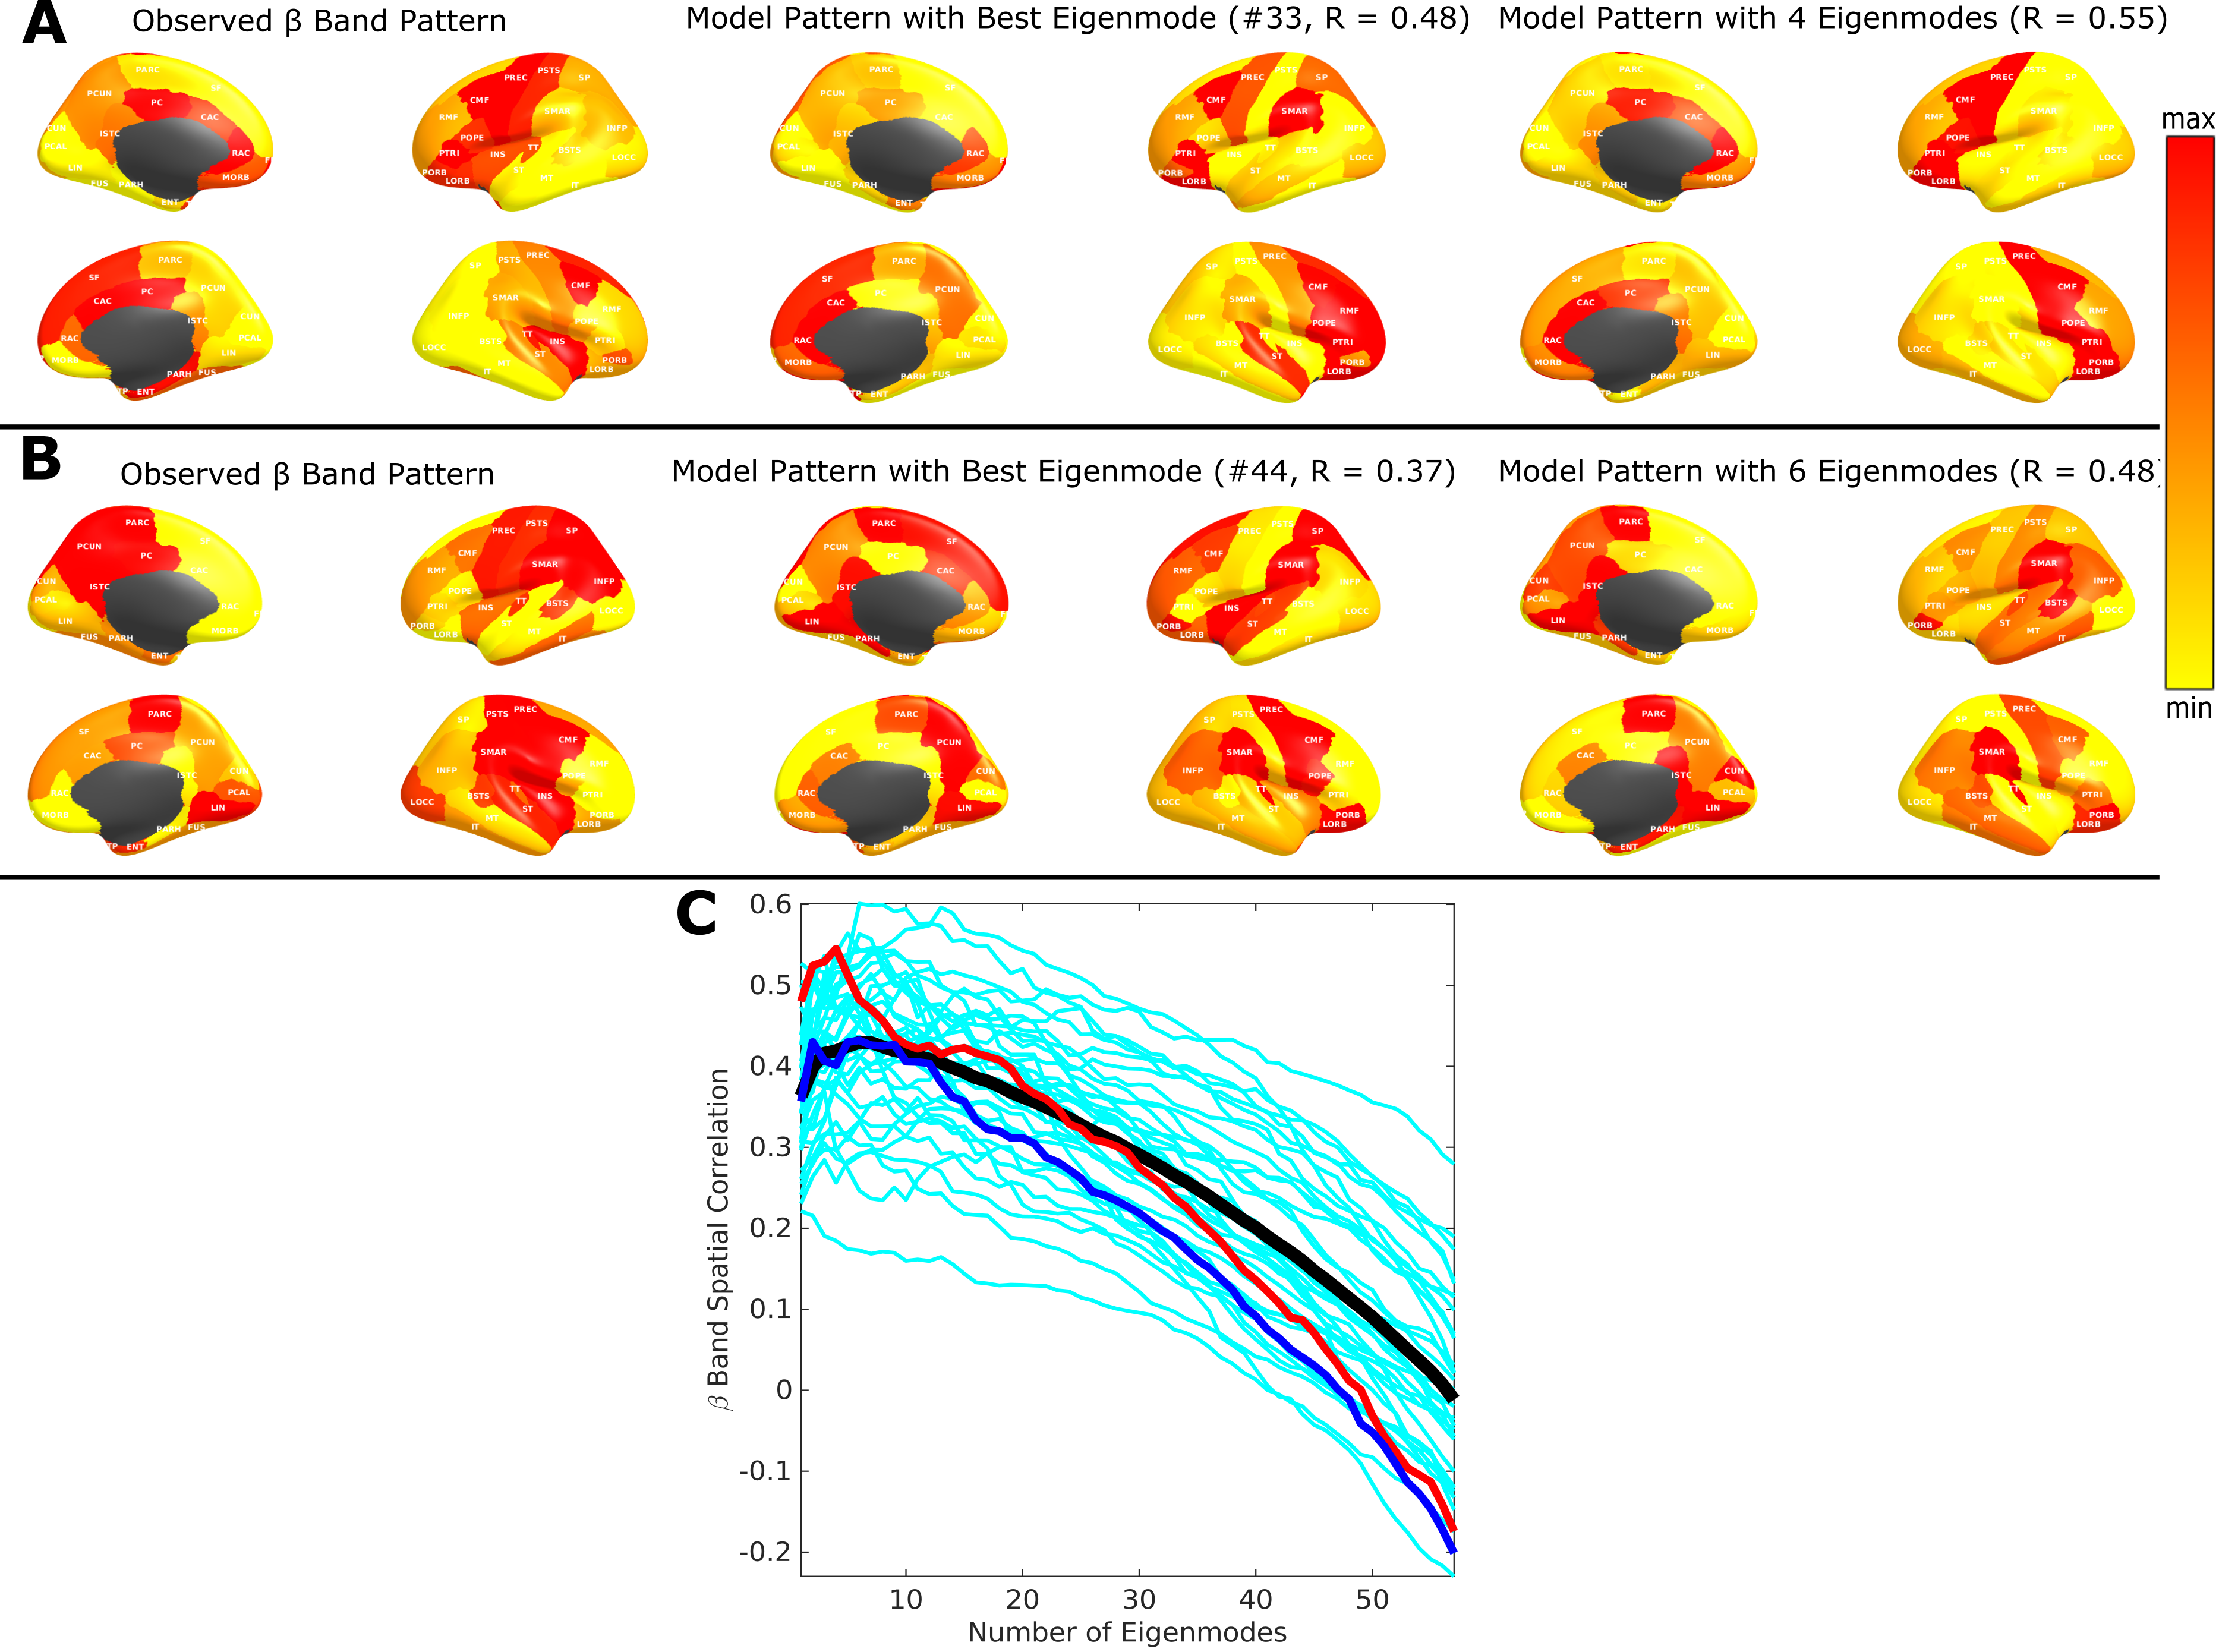
\includegraphics[width=\textwidth]{../figures/chapter5/fig6_beta.png}
    \caption{Beta power spatial distribution depicted by specific spectral graph model eigenmodes.}
    \caption*{Legends and layout is identical to Figure \ref{fig:alpha} but shown for beta band spatial distributions.}
    \label{fig:beta}
\end{figure}

Examples of predicted beta patterns. Empirical beta power
(Figure \ref{fig:beta}, left) is spread throughout the cortex, especially
frontal and sensorimotor cortex. A combination of 4 and 6 best matching
eigenmodes produced the best model match to the source localized pattern
of two representative subjects, respectively, with $R = 0.55$ and $R=0.48$.
Figure \ref{fig:beta}C shows how the spatial correlation changes as more
eigenmodes are used in the "sorted summed" computations, analogous to
that of alpha pattern. Here too a peak is achieved for a small number of
eigenmodes, typically under 10.

\subsubsection{Spatial correlation achieved by the spectral graph model is
significantly higher than alternative models}

\begin{figure}[htbp]
    \centering
    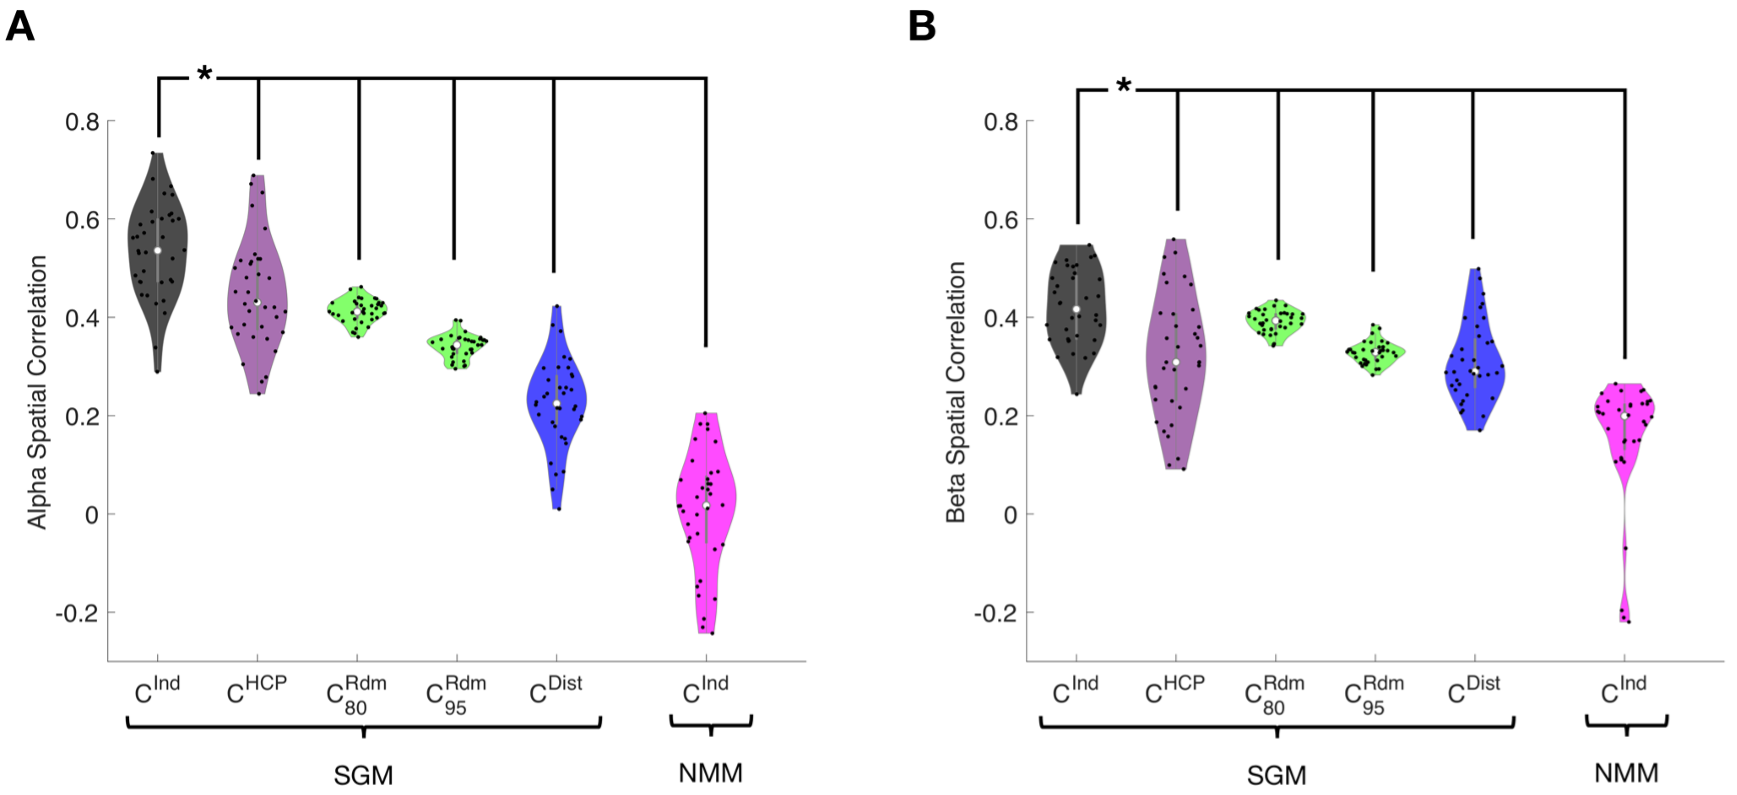
\includegraphics[width=\textwidth]{../figures/chapter5/fig7_spatial.png}
    \caption{Spatial correlation performance of the SGM.}
    \caption*{Distribution of the SGM for all subjects with the best performing eigenmode. (a) Alpha band spatial correlations. (b) Beta band spatial correlations. For both panels, spatial correlations are shown for SGM with subject individual connectomes ($C^{ind}$, black), random connectomes with 80\% and 95\% sparsity (green), geodesic distance based connectome ($C^{dist}$, blue), and finally for a NMM with specific individual connectome (pink). For each scenario, a selection of the best eigenmodes were obtained for spatial correlation calculations separately. Paired t-tests between SGM($C^{ind}$) and all other model simulations show that the SGM with individual connectomes significantly outperform all other models; $p < 0.001$ for all alpha spatial correlations and $p < 0.012$ for all beta spatial correlations.}
    \label{fig:spatial}
\end{figure}

The distribution of peak spatial correlations in the alpha band, using
optimized parameters and individual connectomes of all subjects, is
plotted in Figure \ref{fig:spatial}A. For comparison we show results for four
model types: a) SGM on subject specific individual
connectomes ($C^{Ind}$, black); b) SGM with the HCP
template connectome ($C^{HCP}$ , purple); c) SGM on random
connectomes with 80\% sparsity comparable to individual connectomes or
with 95\% sparsity where the model shows spectral diversity
($C^{Rdm}$ , green); d) SGM on geodesic distance based
connectomes ($C^{Dist}$ , blue); and e) a Wilson-Cowan
NMM with subject specific individual connectome
($C^{Ind}$ , pink). Analogous results for beta band spatial
correlations are contained in Figure \ref{fig:spatial}B. For each connectome
model, a selection of the cumulative best set of eigenvectors were
separately obtained for spatial correlation calculations. Across all
subjects the proposed model, SGM on $C^{Ind}$ , gives
excellent spatial correlations in alpha band (R distribution centered at
0.6) as well as in the beta band ($R$ distribution centered at 0.5).

\subsubsection{Alternate non-linear model}
The Wilson-Cowan neural mass model also did not succeed in predicting the spatial patterns of alpha or beta power, with poor correlations (r centered at 0). This could be because
in our implementation we enforced uniform local parameters with no
regional variability. However, this is the appropriate comparison, since
our proposed model also does not require regionally-varying parameters.
Interestingly, the random connectomes and geodesic distance based
connectome also appear to have some ability to capture these spatial
patterns ($R$ centered at 0.4 and 0.2 respectively), perhaps due to the
implicit search for best performing eigenmodes, which on average will
give at least a few eigenmodes that look like MEG power purely by
chance.

Collectively, we conclude that the graph model is able to fit both the
spectral and spatial features of empirical source localized MEG data,
and that the optimal fits performed on individual subjects occurs at
widely varying subject-specific parameter choices.

\section{Discussion}

The proposed hierarchical graph spectral model of neural oscillatory
activity is a step towards understanding the fundamental relationship
between network topology and the macroscopic whole-brain dynamics. The
objective is not just to model brain activity phenomenologically, but to
analytically derive the mesoscopic laws that drive macroscopic dynamics.
This model of the structure-function relationship has the following key
distinguishing features: \emph{(a) Hierarchical}: the model's
complexity depends on the level of hierarchy being modeled: complex,
non-linear and chaotic dynamics can be accommodated at the local level,
but linear graph model is sufficient at the macro-scale. \emph{(b)
Graph-based}: Macroscopic dynamics is mainly governed by the
connectome, hence linear approximations allow the steady-state frequency
response to be specified by the graph Laplacian eigen-decomposition,
borrowing heavily from \textbf{spectral graph theory}
\cite{auffarth_spectral_2007,Kondor02diffusionkernels,larsen_medical_2006,Ng01onspectral}. \emph{(c) Analytic}: The model is
available in closed form, without the need for numerical simulations.
\emph{(d) Low-dimensional and parsimonious}: Simple, global and
universal rules specified with a few parameters, all global and apply at
every node, are able to achieve sufficiently complex dynamics. The model
is incredibly easy to evaluate, taking no more than a few seconds per
brain and to infer model parameters directly from a subject's MEG data.
The optimized model matches observed spectral and spatial patterns in
MEG data quite well. No time-consuming simulations of coupled neural
masses or chaotic oscillators were needed; indeed, the latter greatly
underperformed our model. We report several novel findings with
potentially important implications, discussed below.

\subsection{Recapitulating regional power spectra at all frequencies}

Our main result is the robust demonstration of the model on 36 subjects'
MEG data. The representative examples shown in Figures \ref{fig:spectra_fit}-\ref{fig:beta} indicate that the graph model recapitulates the observed source localized MEG power
spectra for the 68 parcellated brain regions, reproducing the prominent
alpha and beta peaks. For each region, the model is also able to predict
some characteristics of the full bandwidth power spectra, including what
appears to be an inverse power law fall-off over the entire frequency
range of interest. However, this aspect will be quantitatively
characterized in future work.

We designed a comprehensive parameter optimization algorithm on
individual subjects' MEG data of a suitably defined cost function based
on Pearson R statistic as a way to capture all relevant spectral
features. Using this fitting procedure, we were able to obtain the range
of optimally-fitted parameters across the entire study cohort. As shown
in Figure \ref{fig:violin}A, the range is broad in most cases, implying that there is
significant inter-subject variability of model parameters, even if a
template connectome is used for all. We tested the possibility that a
group-averaged parameter set might also succeed in matching real
spectral data on individuals. But as shown in Figures \ref{fig:spectra_fit}B and \ref{fig:violin}C, this
was found to be a poor choice, supporting the key role of individual
variability of model parameters (but not variability in the connectome).
However, no model is capable of reproducing higher frequencies in the
higher beta and gamma range seen in MEG, since by design and by
biophysical intuition these frequencies arise from local neural
assemblies rather than from modulation by macroscopic networks.

\subsection{Revealing sources of heterogeneity in spatial patterns of brain
activity}

The spatial match between model and data is strongest when the model
uses empirical macroscopic connectomes obtained from healthy subjects'
diffusion weighted MRI scans, followed by tractography. The use of
"null" connectomes - randomized connectivity matrices of varying
levels of sparsity and distance-based connectivity matrices,
respectively, did far worse than actual human connectomes (Figure \ref{fig:spatial}),
supporting the fact that the latter is the key mediator of spatial
patterns of real brain activity. The match was also significantly
different when using a template HCP connectome versus the individual
subject's own connectomes, and when compared to spatial
patterns predicted by an NMM. In conclusion, for the purpose of
predicting the spatial topography of brain activity, it is important to
use individual connectomes and optimized model parameters.

\subsection{Macroscopic brain rhythms are governed by the connectome}

A predominant view assumes that different brain rhythms are produced by
groups of neurons with similar characteristic frequencies, which might
synchronize and act as "pacemakers". How could this view explain why
alpha and beta power are spatially stereotyped across subjects, and why
the alpha signal is especially prominent in posterior areas? Although
practically any computer model of cortical activity can be tuned, with
suitable parameter choice, to oscillate at alpha frequency, e.g.
\cite{liley_alpha_1999,robinson_multiscale_2005,Nakagawa2014,
Deco2012,david_neural_2003,nunez_theoretical_2006,vijayan_thalamocortical_2013}, none of them are able to parsimoniously recapitulate the posterior origin of alpha. Thus the
prominence of posterior alpha might be explained by the hypothesized
existence of alpha generators in posterior areas. Indeed, most
oscillator models of local dynamics are capable of producing these
rhythms at any desired frequency \cite{liley_alpha_1999,david_neural_2003,van_rotterdam_model_1982,liley_spatially_2002,Spiegler2013}, and therefore it is common to tweak their parameters to reproduce alpha
rhythm. Local networks of simulated multicompartmental neurons can
produce oscillations in the range 8--20 Hz \cite{liley_alpha_1999}, and, in
a non-linear continuum theory, peaks at various frequencies in the range
2--16Hz were obtained depending on the parameters \cite{liley_spatially_2002}.
Specifically, the role of thalamus as pacemaker has motivated
thalamocortical models \cite{izhikevich_large-scale_2008,robinson_multiscale_2005} that are capable of resonances in various ranges. Neural field models of the thalamocortical
loop \cite{robinson_multiscale_2005} can also predict slow-wave and spindle
oscillations in sleep, and alpha, beta, and higher-frequency
oscillations in the waking state. In these thalamocortical models, the
posterior alpha can arise by postulating a differential effect in
weights of the posterior versus anterior thalamic projections, e.g.
\cite{vijayan_thalamocortical_2013}. Ultimately, hypotheses requiring local rhythm
generators suffer from lack of parsimony and specificity: a separate
pacemaker must be postulated for each spectral peak at just the right
location \cite{nunez_study_1981}.

An alternative view emerges from our results that macroscopic brain
rhythms are governed by the structural connectome. Even with global
model parameters, using the exact same local cortical dynamics captured
by the local transfer function $H_{local}(\omega)$, driven by
identically distributed random noise $\mathbf{P}(\omega)$, our model
is capable of predicting prominent spectral (Figures \ref{fig:conn_spectra}, \ref{fig:spectra_fit}) and spatial
(Figures \ref{fig:alpha},\ref{fig:beta}) patterning that is quite realistic. This is especially
true in the lower frequency range: indeed, the model is able to predict
not just the frequency spectra in alpha and beta ranges, but also their
spatial patterns -- i.e. posterior alpha and distributed but roughly
frontal beta. Although this is not definitive proof, it raises the
intriguing possibility that the macroscopic spatial distribution of the
spectra of brain signals \emph{does not require spatial
heterogeneity of local signal sources, nor regionally variable
parameters}. Rather, it implies that the most prominent
\emph{patterning of brain activity (especially alpha) may be
governed by the topology of the macroscopic network} rather than by
local, regionally-varying drivers. Nevertheless, a deeper exploration is
required of the topography of the dominant eigenmodes of our linear
model, in order to understand the spatial gradients postulated
previously \cite{robinson_multiscale_2005,vijayan_thalamocortical_2013}.

\subsection{Emergence of linearity from chaotic brain dynamics}

The non-linear and chaotic dynamics of brain signals may at first appear
to preclude deterministic or analytic modeling of any kind. Yet, vast
swathes of neuroscientific terrain are surprisingly deterministic,
reproducible and conserved across individuals and even species. Brain
rhythms generally fall within identical frequency bands and spatial maps
\cite{freeman_simulated_2009,robinson_multiscale_2005,he_temporal_2010}. Based on the hypothesis that the emergent
behavior of long-range interactions can be independent of detailed local
dynamics of individual neurons \cite{shimizu_co-operative_1983,misic_communication_2014,misic_cooperative_2015,destexhe_wilson-cowan_2009,abdelnour_network_2014}, and may be
largely governed by long-range connectivity \cite{abdelnour_estimating_2015,Nakagawa2014,jirsa_spatiotemporal_2002,Deco2012}, we
have reported here a minimal linear model of how the brain connectome
serves as a spatial-spectral filter that modulates the underlying
non-linear signals emanating from local circuits. Nevertheless, we
recognize the limitations of a linear model and its inability to capture
inherent non-linearities across all levels in the system.

\subsection{Relationship to other work}

One can view the proposed generative model as a biophysical realization
of a dynamic causal model (DCM) \cite{daunizeau_dynamic_2011,friston_dynamic_2017,pinotsis_anatomical_2013,razi_construct_2015,pinotsis_linking_2017} for whole brain electrophysiological activity but with very different goals, model
dimensionality and inference procedures.

First, the goal of many prior efforts using DCMs is to examine effective
connectivity in EEG, LFP and fMRI functional connectivity data,
typically for smaller networks\cite{pinotsis_linking_2017,daunizeau_dynamic_2009}, or dynamic
effective connectivity\cite{park_dynamic_2018,van_de_steen_dynamic_2019,preti_dynamic_2017}. Hence, they address the second order covariance structures of brain activity. In particular,
recent spectral DCM and regression DCM models \cite{razi_large-scale_2017,frassle_regression_2017,frassle_generative_2018}
with local neural masses are formulated in the steady-state
frequency-domain, and the resulting whole-brain cross-spectra are
evaluated. The goals of these models are to derive model cross-spectra
that define the effective connectivity in the frequency domain and are
compared with empirical cross-spectra. Based on second-order sufficient
statistics, these models attempt to derive effective connectivity from
functional connectivity data. These DCMs have so far only been applied
to small networks or to BOLD fMRI regime. In contrast, our goal is to
examine the role of the eigenmodes of the structural connectome and
their influence on power spectral distributions in the full MEG
frequency range, and over the entire whole brain. In subsequent work, we
intend to extend our efforts to examining effective connectivity but
such an effort currently remains outside the scope of the work in this
paper. Here, we focus on models that directly estimate the first order
effects of observed power spectra and its spatial distributions and
compare them with empirical MEG source reconstructions. Our primary
motivation is to examine whether spatial distribution of observed power
spectra can arise from graph structure of the connectome, hence our
focus on the effects of model behavior as a function of the underlying
structural connectome -- whether it is individualized, template-based,
uniform, random or distance based. DCM methods have not reported first
order regional power spectra as we do here, nor have they explored how
the structural connectome influences model spectral distributions.

Second, our model is more parsimonious compared to most of these
above-mentioned models which have many more degrees of freedom because
they often allow for regions and their interactions to have different
parameters. Our model parameterization, with only a few global
parameters, lends itself to efficient computations over fine-scale
whole-brain parcellations, whereas most DCMs (with the exception of
recent spectral and regression DCMS\cite{razi_large-scale_2017,frassle_regression_2017,frassle_generative_2018}) are suited
for examining smaller networks but involve large effective connectivity
matrices and region-specific parameters. Furthermore, parameters of our
model remain grounded and interpretable in terms of the underlying
biophysics, i.e. time constants and conductivities. In contrast,
spectral and regression DCM models of cross-spectra have parameters that
are abstract and do not have immediate biophysical interpretation.

The third major difference is in the emphasis placed on Variational
Bayesian inference in DCM. Since our focus was on exploring model
behavior over a small number of global parameters and a set of
structural connectomes (whether anatomic or random) of identical
sparsity and complexity, it was sufficient to use a \emph{maximum a
posteriori} (MAP) estimation procedure for Bayesian inference of our
global model parameters with flat non-informative priors with
pre-determined ranges based on biophysics. Like most DCM efforts our
model can be easily be extended to Variational Empirical Bayesian
inference for parameter estimation, for instance to compute a full
posterior of the structural connectivity matrix. In such a formulation,
we can assume that the observed structural connectome will serve as the
prior mean of the connectivity matrix. We reserve such extensions to our
future work with this spectral graph model.

\subsection{Other limitations and extensions}

The model currently examines resting-state activity, but future
extensions will include prediction of functional connectivity,
task-induced modulations of neural oscillations and causal modeling of
external stimuli, e.g. transcranial magnetic and direct current
stimulation. The current implementation does not incorporate complex
local dynamics, but future work will explore using non-white internal
noise and chaotic dynamics for local assemblies. This may allow us to
examine higher gamma frequencies. Although our model incorporates
latency information derived from path distances, we plan to explore
path-specific propagation velocities derived from white matter
microstructural metrics such as axon diameter distributions and myelin
thickness. Future work will also examine the specific topographic
features of the structural connectome that may best describe canonical
neural activity spectra. Finally, we plan to examine the ability of the
model to predict time-varying structure-function relationships.

\subsection{Potential applications}

Mathematical encapsulation of the structure-function relationship can
potentiate novel approaches for mapping and monitoring brain diseases
such as autism, schizophrenia, epilepsy and dementia, since early
functional changes are more readily and sensitively measured using fMRI
and MEG, compared to structural changes. Because of the complementary
sensitivity, temporal and spatial resolutions of diffusion MRI, MEG, EEG
and fMRI, combining these modalities may be able to reveal fine
spatiotemporal structures of neuronal activity that would otherwise
remain undetected if using only one modality. Current efforts at fusing
multimodalities are interpretive, phenomenological or statistical, with
limited cognizance of underlying neuronal processes. Thus, the ability
of the presented model to quantitatively and parsimoniously capture the
structure-function relationship may be key to achieving true
multi-modality integration.